\documentclass[12pt]{article}
\linespread{1.5}
\pdfminorversion=6

\usepackage[english]{babel}
\usepackage{booktabs}
\usepackage{bookmark}
\usepackage{tabularx}
\usepackage{caption}
\usepackage{float,color}
\usepackage{graphicx,scalerel}
\usepackage{hyperref}
\hypersetup{colorlinks,linkcolor=black,urlcolor=blue,citecolor=black}
\usepackage{amssymb}
\usepackage{amsmath}
\usepackage{bbm}
\usepackage{placeins}
\usepackage[format=hang,font=normalsize,labelfont=bf]{caption}
\usepackage[margin=1in]{geometry}
\usepackage{url}
\usepackage{listings}
\usepackage{amsxtra}
\usepackage{setspace}
\newcommand{\Rho}{\mathrm{P}}
\usepackage{authblk}
\usepackage{graphicx}
\usepackage[flushleft]{threeparttable}
\usepackage{longtable}
\usepackage{threeparttablex}
\usepackage{multirow}
\usepackage{array}
\usepackage{tikz}
\usepackage{csquotes}

\usepackage{epigraph}
\setlength \epigraphwidth {\linewidth}
\setlength \epigraphrule {0pt}
\AtBeginDocument{\renewcommand {\epigraphflush}{center}}
\renewcommand {\sourceflush} {center}

% Bibliography stuff
\usepackage[
hyperref=true,
giveninits=true, % render first and middle names as initials
uniquename=init,
maxcitenames=3,
maxbibnames=99,
style=authoryear,
dashed=false, % re-print recurring author names in bibliography
natbib=true,
useprefix=true, % for inclusion of 'de' 'da' in surname
urldate=long,
backend=biber,
style=apa]{biblatex}
\addbibresource{bibliography.bib}

% Scale hats and bars (e.g. \wh{x})
\newcommand\wh[1]{\hstretch{2}{\hat{\hstretch{.5}{#1}}}}
\newcommand\wb[1]{\hstretch{2}{\bar{\hstretch{.5}{#1}}}}

% custom table functions
% indents second level entries
\newcommand{\indentrow}[1]{\quad #1}

% adds space above row
\newcommand{\customlinespace}{\addlinespace[.1cm]}

% command for all table/figure notes
\newcommand{\Fignote}[1]{
	\begin{tablenotes}[para,flushleft]\footnotesize
		\textit{Note}: #1
	\end{tablenotes}
}

% stars
\newcommand{\sym}[1]{\rlap{#1}}

% note addendem for regression tables
\newcommand{\Regnote}{Standard errors in parentheses are robust to heteroskedasticity. ***, **, and * indicate significance at the 1, 5, and 10 percent critical levels, respectively.}

% Flowchart helpers
\usetikzlibrary{shapes, arrows, positioning, trees}


% *****************************************************************
% Title page stuff
% *****************************************************************

\title{The effect of a supplementary video book on learning in intermediate microeconomics}
\author{Melissa Famulari}
\author{Zachary A. Goodman\thanks{mfamulari@ucsd.edu and zgoodman@ucsd.edu. The authors thank the students who took intermediate microeconomics in the fall of 2018 and 2019 for participating in this study. We also thank UC San Diego's Teaching + Learning Commons for helping provide and anonymize the data used for analysis. Finally, we thank the applied microeconomics group at UC San Diego for their helpful feedback on the experimental design and analysis. This research was approved under UC San Diego's Human Research Protections Program (IRB approval 170886 in fall 2018 and 2019). The paper investigates the use of Intermediate Microeconomics Video Handbook (IMVH) video lectures by UC San Diego students, some of which were developed by one of the authors, in collaboration with UC San Diego and the UC Office of the President. UC San Diego currently owns the rights to distribute the IMVH. The videos lectures were provided to the subjects at no charge and neither author has a direct financial interest in the distribution of the IMVH within the University of California. As of fall 2020, one of the authors has a financial interest in the distribution of the IMVH outside of the University of California.}}
\affil{University of California, San Diego}
\date{This version: March 2021} % TODO: add link to most recent version


% *****************************************************************
% Begin Paper
% *****************************************************************

\begin{document}

% remove ``Abstract" from above abstract
% \renewcommand{\abstractname}{\vspace{-\baselineskip}}

\maketitle
\begin{abstract}
	In this paper we estimate the effectiveness of a novel video-based textbook replacement for intermediate microeconomics, the Intermediate Microeconomic Video Handbook (IMVH), on learning outcomes. In a field experiment involving nearly 400 students, we randomly assigned a grade-based incentive that induced treatment students to watch over 60\% more videos than did control students. We observe significant reduced form effects: being assigned treatment caused students to score 0.18 standard deviations higher on midterm and final exams. Using an instrumental variables approach, we estimate that the marginal hour of video content increased exam scores between 0.05 and 0.15 standard deviations. We rule out large negative spillover effects to other courses taken concurrently, and we observe persistent take-up of the IMVH in the subsequent quarter when direct incentives to watch videos were removed.
\end{abstract}

% *****************************************************************
% Introduction
% *****************************************************************

\section{Introduction}

\epigraph{\textit{``You expect me to read the textbook? Ha!''}}{--- Anonymous student}\bigskip

Every year, university students spend tens of thousands of dollars on tuition and hundreds of hours studying, in large part, to learn. Instructors can help their students learn more efficiently by providing and recommending pedagogical tools that have high returns per unit time and financial cost. Despite the value to students and instructors, little empirical work exists that estimates the effectiveness of different learning technologies \parencite{aws2015}.

In this paper, we measure the impacts of one such technology, the Intermediate Microeconomic Video Handbook (IMVH), on outcomes in an intermediate microeconomics course. The IMVH was designed to \textit{supplement} lecture as an audiovisual version of a conventional course textbook. Part of the impetus for creating the IMVH was a discussion with a student who described her inability to read the course text, not because of poor reading skills, but because she did not find the text engaging enough to command her attention. We hypothesized that modern students, who have had unprecedented exposure to electronic media, may find videos more engaging and, perhaps, more effective at building human capital.

Besides higher engagement than with conventional texts, the IMVH and video-based learning tools more broadly are of value to university educators and their students for four additional reasons. First, videos carry near-zero marginal cost and are accessible anywhere via internet, helping reduce financial and geographic barriers to high-quality educational materials. Second, video platforms can help students track what content they have already studied and what content they have yet to cover. Third, features embedded into videos, such as searchable captions and timestamps, can help students locate the information they are seeking faster. Finally, the perceived low cost of watching a brief video may be easier to overcome than perceived higher costs of other studying methods, potentially leading to more frequent studying, which decades of psychological research has demonstrated leads to more long-term learning than does cramming \parencite{kornell2009, cpvw2006}.

Ultimately, the beneficial features of video-based learning tools are of value only if they can improve student learning outcomes, an empirical question we seek to answer in this paper. To estimate the effects of the IMVH, we administered a field experiment involving nearly 400 undergraduates enrolled in the same one-quarter-long microeconomics course over two years. Of note, these students all scored below the median on the first midterm exam, thereby making manifest a need to adjust studying habits, and perhaps standing to gain the most from an intervention that targets studying. We randomly assigned a grade-based incentive to half of the sample to encourage take-up of the IMVH, which was made available to all students in the experiment, allowing identification of intent to treat (ITT) effects and local average treatment effects (LATEs) while maintaining equitable access to learning resources. We tracked video watching at the student level using the software platform that hosts the IMVH. We observe grades, GPA, and video watching in both the term of the experiment and the subsequent term.

The first-stage impact of the exogenous encouragement on video watching is significant and substantial. Students who receive the grade-based incentive watch over 28\% more unique videos by the second midterm and 63\% more unique videos by the final exam, or about 1.1 and 3.4 hours of content, respectively, than did their control peers. We find large reduced-form effects of treatment on exam scores: being assigned treatment (ITT) increases midterm and final exam scores by about 0.18 standard deviations. Our estimates imply that the marginal hour of videos watched increases exam scores (LATE) by between 0.05 and 0.16 standard deviations.

We interpret our results through a theoretical framework in which students, who value grades and leisure, have potentially incorrect priors about the returns of different studying methods. We do so not to test theory, but rather to help educators understand the potential welfare implications of providing students with a learning technology and paternalistic incentive structure like the one studied. Although we observe that treatment students performed better on course assessments, for welfare analysis one must consider where the time watching videos came from: leisure, work, student organizations, studying for other classes, studying for present class using other methods, etc. If students must reduce time allocated towards leisure or studying for other classes so they can watch more videos, then the welfare impacts of requiring videos could be negative depending on the students' preferences. On the other hand, if the videos are more productive than the next best studying technology, then requiring videos could be utility enhancing.

To better understand the spillover effects of treatment, we examine other forms of studying including class attendance, visits to a tutoring center (specific to this course), and interacting with the class discussion board. We do not find any statistically significant changes in any observed studying method, and we can rule out large changes. In nearly all cases, treatment students used other studying methods at directionally \textit{greater} rates than did their control peers. We also investigate spillovers to other courses taken during the term of the experiment and similarly find that treated students perform directionally \textit{better} than their control peers. Though not statistically significant, we can rule out large negative effects, suggesting that treatment did not cause students to dramatically substitute away from studying for other courses.

An important piece to the welfare puzzle is whether treatment students continue to use the IMVH at higher rates after exogenous incentives are removed. Persistent take-up in the absence of external prodding provides some confidence that students, now with updated priors, value the technology. Fortunately, we can observe video watching in the subsequent microeconomics course in the term following the experiment. Despite there being no direct incentives to watch videos in the subsequent course, treatment students persistently watched more videos than did control students, about 8 - 10 more unique videos, or 1.2 - 1.5 more hours of unique content. Our sample in the subsequent term is nearly half the original size, so we lack power to precisely estimate effects on exam scores; however, our confidence intervals include effect sizes consistent with those observed in the experiment term.

Collectively, we interpret our findings as evidence that requiring the IMVH is a net positive on underperforming students' academic achievement, both in the quarter of the experiment and beyond. Though formal welfare analysis is beyond the scope of this paper, we present suggestive evidence that requiring the IMVH is unlikely to be substantially utility harming, if not utility enhancing. We believe our findings justify paternalistic incentive structures in settings where a large portion of the class is at risk of failing and the instructor has more information about the usefulness of a novel learning technology than do her students.

% novelty of study design? Using poor performance on early-stage assessment to determine experiment eligibility. Use of separate curves to maintain fairness, a common argument against conducting RCTs in academic settings. Applicable in large lectures where anticipated effect sizes are large (>0.15 standard deviations).

The rest of the paper is organized as follows. Section \ref{models} presents competing models of studying behavior that may explain the observed phenomena. Section \ref{background} provides background on existing related literature. Section \ref{studydesign} describes the study design. Section \ref{results} presents the results of the experiment, and Section \ref{discussion} discusses those results. Section \ref{conclusion} concludes.

% *****************************************************************
% Background
% *****************************************************************

\section{Related Literature} \label{background}

Students have many time-consuming activities to help them learn including attending class, watching recorded lectures, reading the textbook, doing homework or practice exams, or attending tutoring labs, and there are many empirical challenges to estimating the causal effects of a learning activity. First, a student's decision to use a study method is likely influenced by unobservable student characteristics, such as motivation or ability, that also likely affect student exam performance. To estimate causal effects, researchers must address nonrandom selection into using the study method. Second, motivated students often visit instructors seeking help improving their study strategies after a negative exam shock which suggests ``dynamic selection" into the use of a study method and has been found empirically by \textcite{oettinger2002}, \textcite{ko2005}, \textcite{ss2008}, \textcite{bo2012} and \textcite{bo2015}.\footnote{\textcite{oettinger2002} finds that students close to a grade threshold before the final exam perform better on the final. \textcite{ko2005} show that students reduce the number of hours they study after getting higher midterm scores. \textcite{ss2008} find that IV estimates of studying on grades are much larger than OLS and provide suggestive evidence that students increase effort in semesters when semester-specific elements of grades are low. In two papers, \textcite{bo2012} and \textcite{bo2015} find that the difference between a student's expected and actual grade on an early assessment is positively correlated with a change in their study hours (after-assessment study hours minus before-assessment study hours). This suggests that students with a negative exam shock (actual grade worse than expected) may respond by increasing their study hours.}
Dynamic selection means including student fixed effects in class performance regressions will not uncover the causal effect of a study method. Third, study methods may be substitutes or complements in student learning and experimental inducements to use one study strategy may affect student use of another. In these cases, even randomized experiments will not identify the causal effects of a particular study method but will instead identify the causal effects of a study policy and all of the changes in student behavior caused by that policy.\footnote{While the causal effects of an educational policy are useful for educators considering how to design their classes they are less useful for students wanting to know the most productive use of their study time. We should also point out that instructors may find learning transmission methods substitutable or complementary. As an example, in \textcite{msc2019} many instructors report that lecture capture, where lectures are recorded and made available to students, changed the way they lectured in the classroom. Experiments randomly assigning students to classes taught one way versus another will not identify the causal effect of a study method if other aspects of learning transmission are simultaneously changed.} %Fourth, the existence of the resource may change how the instructor teaches. For example, several papers discuss how lecture capture changes the way instructors lecture. Again, experiments randomly assigning student to classes taught one way versus another will not identify the causal effect of a study method if other aspects of learning transmission are changed.
Finally, experimental inducements to use a study method may change the total time devoted the course. In this case, experiments jointly test the effectiveness of a particular learning method and devoting more (or less) time to the course.

% Our study uses a randomized control trial as well as a RD approach which solves issues (1) and (2). Since we use within-class randomization, we solve issue (4). Our study does not solve issues (3) and (5), however, we have empirical evidence on a large number of alternative study methods and test if the inducement to use the video book affected these other study methods to shed light on issue (3) and we have survey data on study time for the course for a selected sample of students which we use to test whether total study time for the course differs across treated and control students to shed light on issue (5).

We focus our review on studies that use experiments or quasi-experiments (regressions discontinuity or instrumental variables) to explore the effects of learning acquisition that take students' time.\footnote{Using the IMVH takes student time, so we focus on research that estimates the causal effects of other time-consuming study methods. We do not include research that examines how to make studying methods more productive, though the intensive margin of pedagogical tools is certainly an important area of study with potentially clearer welfare implications.} We organize these studies into two broad groups: \textit{guided-study}, such as attending lecture, tutoring labs, and discussion sections/tutorials/recitations (small problem-solving sessions offered by TAs), or \textit{self-study}, which includes doing homework, practice exams and watching recorded lectures. \textcite{km2003} use student-reported travel time to campus as an instrument for lecture attendance. They find no selection bias and so find the usual positive relationship between lecture attendance and exam grades in OLS regressions. \textcite{dgm2010} analyze a policy where lecture attendance was voluntary before the midterm but after midterm grades were posted, lecture attendance was required for students who scored below the median. At the threshold there was a 36 percentage point increase in post-midterm attendance. Using a regression discontinuity approach to estimate the effects of attendance on the final exam, they find a 10 percentage point increase in student attendance led to a .17 standard deviation increase in final exam score. \textcite{jcjao2015} randomly assign 725 students taking introductory microeconomics students to twice per week and once per week lecture formats to identify the effects of classroom time in classes that are well-supported with online content (videos, quizzes, posted PowerPoint lectures, etc.) Students in the twice per week format scored 0.21 standard deviations higher on the midterm and 0.14 standard deviations higher on the final exam. Finally, \textcite{tlad2020} randomly assign students to either weekly or bi-weekly grading of in-class clicker questions. Weekly grading increased student lecture attendance by 11 percent but not student-reported self study hours. Course grades were 6.31 percent higher for students randomly assigned to weekly grading and the effects of weekly grading were much stronger if the student preferred bi-weekly grading, had lower prior GPAs and lower self-control scores.\footnote{\textcite{cl2008} randomly omit material from lecture from a randomly chosen class and find students who heard the material did better on related multiple choice questions. However since both treatment and controls are in lecture, this study abstracts from the time costs of attending lecture and we focus on empirical studies exploring study methods that take time.}

\textcite{ans2012} study discussion section attendance. Since students are randomly assigned to sections and section attendance is influenced by day of week and time of day, the authors use time of a student's section as an instrument for attendance. They find no effects of section attendance for most students, but for students in the top quantiles, missing 10 percent of sections caused a 1 percentage point performance loss. \textcite{kow2020} also examine the effects of section but like \textcite{dgm2010} study a university-wide attendance policy focused on students who reveal themselves as poor performers. The university required 70 percent section attendance in the second year for students whose first year GPA was below a threshold. They find students just below the threshold attended 50 percent more sections and lectures but reported no significant difference in total study hours (lectures plus section plus self study). Interestingly, the authors report zero overall effect on grades and a substantial \textit{negative} effect in classes where attendance was optional for students above the threshold. \textcite{bs2013} examine attendance for lecture and discussion sections combined. Using student residence as an instrument and controlling for self study hours, the authors find no significant effect of attendance on grades for most courses but significantly positive effects for quantitative courses.

At many universities, students can visit tutoring labs for help learning the material covered in lecture or discussion sections. \textcite{mgm2010} find athletes are significantly more likely to attend peer tutoring labs, which the authors attribute to frequent reminders from coaches. Using one's status as an athlete as an instrument for tutoring hours, they find significantly positive effects of peer tutoring: attending tutoring one hour per week over a 14-week semester increases a student's final grade by one letter. Collectively, the aforementioned studies on the effects of guided instruction, across all types, consistently find that student performance is improved, but only if students do not substitute self-study time for guided instruction.

Turning to the effectiveness of self-study, \textcite{ss2008} examine 210 Berea College students who were randomly assigned a roommate. Students whose roommate brought a video game to college earn lower grades and spend less time studying. They authors instrument for study time using presence of a roommate with a video game and find that an additional hour of studying per day increases GPA by 0.36 points. On the other hand, \textcite{oppp2019} randomly assign first year economics students at three different institutions to a variety of low-touch interventions to increase study hours (planning studying schedules, information about the value of studying, and weekly reminders about study plans) and find no effect on grades, credit accumulation, or retention despite increasing student's self-reported study hours. \textcite{cgpr2020} also explore a low touch intervention, having students set goals on the number of practice exams they will complete, and find those randomly assigned to set task-based goals completed 0.102 standard deviations more practice exams and increased total course points by .068 standard deviations.

\textcite{ts2012} examine the causal effects of homework by randomly assigning whether or not homework would contribute to students' grades in a Principles of Economics class. The authors find significant positive effects of homework on the first midterm but no effects on the final exam. \textcite{gr2013} conduct a similar experiment, randomly assigning students to a ``homework required" group, for whom homework was worth 10\% of the final grade, and ``homework not required" group, for whom exams were correspondingly upweighted. The authors find that 90\% of treatment students completed 7 or more homework assignments compared to 6\% of control students and on average scored higher on exams. As a whole, the research on the causal effects of self-study is mixed and ranges from no significant effect on exams to large positive effects on GPA. While there is some evidence that self-study may matter for early assessments, more research is warranted.

Finally, we review the research on lecture capture and flipped classrooms, both of which have aspects similar to the IMVH. Lecture capture provides students with recordings of lectures, which students may use as a substitute for lecture, to rewatch for enhancing understanding, or as review before exams. By necessity, recorded lectures cannot be made available to students before lecture and hence cannot help students prepare for lecture. To the best of our knowledge, there is no experimental or quasi-experimental research estimating the causal effects of lecture capture. In flipped classrooms, students watch material in advance of class and work on problems during class where instructional staff are available to answer questions. Two RCTs involving students at U.S. military academies shed some light on the effectivenes of flipped classrooms in university settings. In a small RCT (137 students in 7 sections of an introduction to economics course), \textcite{wbi2018} assign lecture type (flipped vs traditional) to randomly chosen topics and randomly chosen instructors. They find that the flipped classroom increases exam scores by 0.16 standard deviations for medium-term assessments but no effect on short-term exams or the comprehensive final. In a larger RCT (1,328 students in 80 course sections and 29 instructors) across two courses, Principles of Economics and Introductory Calculus, \textcite{sgmy2021} randomly assign half of sections to cover a particular course topic using the flipped model and half to cover the topic using a traditional model. The authors find significant positive effects on a low-stakes quiz but no effects on the final exam.

%Other researchers have investigated using technology to improve learning. \textcite{abbm2020} conduct an experiment in Botswana during the COVID-19 pandemic and find that text messages and phone calls deployed as low cost, scalable learning technologies improved test scores by 0.16 to 0.29 standard deviations.

% comparison of incentivizing goals more generally? Fryer 2011 QJE reviews several large ($millions) in K12 experiments

% Effect of Setting Goals: \textcite{cgpr2020}, hereafter CGPR, explore the effect of having students set goals on class performance. They find that setting \textit{task-based} goals of completing a specific number of online practice exams improves student performance on exams. Those randomly assigned to set task-based goals completed 0.10 standard deviations more practice exams and increased total course points by 0.07 standard deviations. The authors found no significant effect of setting \textit{performance-based} goals of achieving specific grades in the course or on exams on total course points. In the present study, we set for the students a \textit{task-based} goal of watching a specific number of videos. Our intervention differs from that of CGPR in two important ways. First, the instructor, not the students, set the value of the goal. Second, we motivate students to watch videos through a quantifiable grade incentive instead of appealing to psychological forces such as internal commitment devices.

% *****************************************************************
% Study design
% *****************************************************************

\section{Study Design} \label{studydesign}

\subsection{Description of the sample and institution}

We conducted the field experiment in an undergraduates intermediate microeconomics course taught during fall 2018 and fall 2019 by one of the authors. The university is a large, diverse and selective public research university in the United States.\footnote{The Carnegie Classification of Institutions of Higher Education classifies the university as an R1 (very high research activity) university. For the 2017-2018 academic year, the undergraduate student body shared the following demographics: 49.1\% female, 50.6\% male; 75.0\% in-state, 5.5\% out-of-state, and 19.5\% international; 59\% students of color; 28.6\% majoring in the social sciences, 26\% of which major in Economics. Among newly admitted students, about one-third were transfer students, and average SAT scores were 652 and 605 for math and critical reading, respectively. About 34\% of students are the first in their family to attend a four-year university.} At this institution, intermediate microeconomics is a three-quarter sequence required for students majoring in Economics. The experiment was conducted in the first course of the sequence, \textit{Micro A}. We also observe grades and video watching in the second course of the sequence, \textit{Micro B}, the same instructor during both the winter 2018 and winter 2019 quarters. Both Micro A and B instructors created half of the videos relevant to their course in the IMVH.

% details about students themselves, like demographics?

The structure is similar across the three courses in the Micro sequence. Students have the option to attend one of two lectures offered back to back twice per week, each lasting about 90 minutes. Two midterm and final exams are held at a common time outside of lecture. In addition to lecture, students have access to weekly one-hour discussion sections run by graduate teaching assistants (TAs) who are all Economics PhD candidates, including, at the time, one of the authors. In lieu of office hours, the TAs and Undergraduate Instructional Assistants (UIAs) staff a tutoring lab open between three and four hours per day, six days per week. Students may also attend weekly Supplemental Instruction (SI) sessions offered by undergraduates majoring in Economics and trained by the university in SI. Besides the IMVH, students have access to a variety of online learning resources including a discussion board moderated by the instructional team, four years of previous exam questions, weekly ungraded problem sets, and semi-weekly graded online quizzes.

% blurb about the curriculum? Are lectures recorded? My lectures were not recorded.

% why might the results be externally valid, or at least more interesting beyond UCSD? Intermediate micro is a required course in all econ programs and tends to be challenging at all institutions (this is why Office of President funded the IMVH and we got support for this project from faculty from every across the UC). This is also why UCSD offered to support our classes with supplemental instruction--I could see if the other UCs also support intermediate micro. Another argument we could make is that there are many hard, required courses like interm micro in STEM and people have been interested in determining how to help students succeed. Another tact we could take is to argue is the incentive aspect--a small grade incentive worked rmarkable well to encourage increased effort among at-risk students. Further, that increased effort improved performance, possibly because the IMVH was a particularly effective study tool but it may also be that any added time engaging with the course would have helped (joint test point). We may want to point out somewhere that course material that is relatively fixed may be best to create into a video book so do not have to modify much over the years (which adds to the cost).

Students were told about the experiment during the first lecture and provided an informed consent form in the syllabus. At any time during the quarter, students could opt out of having their data included in the analysis.\footnote{Students could opt out via an online form visible to a third party university organization so that neither the instructor nor research team could observe which students elected to opt out.} Students below the age of 18 at the start of the course as well as students enrolled via the university's extension program were removed from the analysis dataset.\footnote{Students under the age of 18 were excluded per IRB protocol. We exclude extension students because of their potentially very different preparation for the course and our inability to observe pretreatment covariates and outcomes outside of Micro A.} Ultimately, four students under 18, five extension students, and seven students who opted-out were removed from the analysis dataset, leaving a sample of 850 students.

There are two unique demographic features of the class worth noting. First, many non-econ majors take the class to either satisfy general education requirements or to explore majoring in economics. As there are many students in the experiment on the margin of majoring in economics, an important outcome is the likelihood the student takes Micro B. Second, about 37\% of the class is transfer students, for whom the class is not only their first experience with upper division coursework at a four-year research university, but also typically their first time taking classes under the faster-paced quarter system.\footnote{Community colleges, the most common previous institution for transfer students, are on the semester system in the state of the university.} We examine treatment effect heterogeneity to understand whether transfer students might differentially benefit from the IMVH.

\subsection{Description of the IMVH}

The Intermediate Microeconomics Video Handbook (IMVH) is a collection of 220 short videos that cover the material in a year-long intermediate microeconomics course sequence.\footnote{A preview of the IMVH can be found at \url{https://iti.ucsd.edu/IMVH_Misc/Promo/IMVHPromo.html}.} The videos, designed as a complement to both lectures and the course textbook, include graphical and verbal intuition as well as formal algebraic and calculus-based definitions and proofs.

The videos were created by six UC San Diego faculty members with professional videographer and production support. Many videos utilize the ``learning glass," an innovative presentation technology where instructors write with neon markers on a large sheet of glass that has lights embedded along the glass edge to make the colors pop. The remaining videos feature faculty superimposed in front of slides that are often written on during the presentation. Videos are closed captioned and were checked by graduate students for accuracy.

Given the complexity of the material, the IMVH was developed with several key objectives in mind. First, the web interface is clean and simple to not distract from the content. Second, to help students find material quickly, videos can be accessed via either the table of contents or the index, each video contains time stamps of the concepts therein and captions are searchable, which allow the student to jump to the part of a video containing the searched-for word. Finally, the videos are organized by content area (e.g., consumer theory, producer theory, etc.) that help students understand where various topics ``live" in intermediate microeconomics.

While we do not know of another textbook completely comprised of videos, the IMVH is similar to the Khan Academy website, lecture podcasts, and textbook websites that incorporate instructional videos. Besides the engaging viewable nature, the IMVH differs from a traditional textbook in that the instructors explain, graph, and derive mathematical results in much the same way one would in a conventional lecture. However, the IMVH differs from lectures in that students control the pace: they can rewatch, speed up, or slow down the videos. Another difference is the ability to read captions and the reduced demand on the instructor's time.

% alternative checkmark option:
% \def\checkmark{\tikz\fill[scale=0.4](0,.35) -- (.25,0) -- (1,.7) -- (.25,.15) -- cycle;}

\begin{table}
	\caption{Comparison of information transmission formats} \label{tech_comparison}
	\centering
	\begin{tabular}{|c*{4}{|>{\centering\arraybackslash}m{0.1\linewidth}}|}
		\hline
		Feature & Lecture & eText-book & Lecture Capture & IMVH\\
		\hline
		Instructor's time used & \checkmark & & &\\
		Instructor-learner interaction & \checkmark & & &\\
		Learner-learner interaction & \checkmark & & & \\
		Readable & & \checkmark & ? & \checkmark \\
		Scalable & ? & \checkmark & \checkmark & \checkmark \\
		Searchable & & \checkmark & & \checkmark \\
		Skimmable & & \checkmark & & \checkmark \\
		Stoppable & ? & \checkmark & \checkmark & \checkmark \\
		Watchable & \checkmark & & \checkmark & \checkmark \\

		\hline

	\end{tabular}
	\label{infotransmission}
\end{table}

Table \ref{tech_comparison} presents a classification of some options to present course material to students.\footnote{This table is a modification of the classification Martin Osborne proposed to one of the authors in an e-mail correspondence.} The IMVH differs from a traditional textbook because instructors verbally explain, graph and derive mathematical results in much the same way one would in a lecture. The primary benefit of lecture over the IMVH is that students can stop the instructor and get an answer as soon as they are confused, or wonder about a connection of the material with their lives or other courses, or want to know if they are right about an extension of the material, etc. Further, student questions may have import externalities for the learning of other students in the class. There is also an important social aspect of lectures as students can interact with each other before, during and after lecture. Students cannot ask questions or interact with other students during an IMVH lecture. Some of the advantages of the IMVH over lecture are first, students control the IMVH in that they can rewatch, speed up, or slow down an IMVH video. Second, compared to a large lecture hall, all students can clearly see and hear the IMVH presentation. Finally, the IMVH is closed-captioned, which may be particularly useful when English is not the first language of the instructor and/or the student. The IMVH differs from lecture capture because the IMVH videos are much shorter, averaging under ten minutes. The IMVH website is well organized so students can see where the topic ``lives" at all times. A useful feature of recorded lectures is they have course administration information which the IMVH does not have. However recorded lectures may also include components that do not work well when recorded, such as group work or class discussion.

\subsection{Experiment Design} \label{expdesign}

The experiment began four weeks into the ten week term following grading the first midterm exam. All students who scored above the median on the first midterm, the \textit{Above median} arm, and half of students who scored below the median, the \textit{Control} arm, were assigned a conventional grading scheme that places weight only on exams and quizzes. We assigned the remaining half of students below the median to the \textit{Incentive} arm, whose grading scheme allots four percentage points conditional on watching at least 40 of 48 eligible videos in the IMVH.\footnote{Watched in standard speed, 40 videos would require students to spend between 5.5 and 7.1 hours, depending on the length of videos chosen (on average 9.7 minutes in length each). Watching all 48 incentivized videos in standard speed would require just shy of eight hours.} These 48 videos review new class content since the first midterm that could be assessed in the second midterm and final exam. Students could still view the remaining 26 course-relevant videos, and as they could have helped students on the cumulative final exam, we include them in our measures of video watching despite not counting towards the grade incentive.

The two different grading schemes are outlined in Table \ref{gradescheme}. Notably, the four percentage points come at the expense of reduced weight placed on the first midterm score, which had already occurred at the time of treatment assignment. Hence, at the time of treatment assignment, the video incentive is the sole forward-looking difference between treatment arms.

\begin{table}
	\caption{Grade scheme by treatment arm. \textit{Control} represents same grade scheme as \textit{Above median}. Differences between the two grade schemes in bold.}
	\centering
	\begin{tabular}{ c|c|c }
		Assessment & Incentive & Control \\
		\hline
		$>$40 videos & \textbf{4\%} & \textbf{0\%} \\
		Midterm 1 & \textbf{18\%} & \textbf{22\%} \\
		Midterm 2 & 22\% & 22\% \\
		Final Exam & 50\% & 50\% \\
		Math Quiz & 1\% & 1\% \\
		Best 5 of 6 Quizzes & 5\% & 5\% \\
		\hline
		Total & 100\% & 100\% \\
	\end{tabular}
	\label{gradescheme}
\end{table}

To improve balance between \textit{Incentive} and \textit{Control} arms and increase statistical power, we assigned students to treatment arms using paired randomization \parencite{ai2017}, matching students by their first midterm scores before randomly assigning one member of each pair to \textit{Incentive} and the other to \textit{Control} (further details on treatment assignment can be found in Appendix \ref{a_randomization}). We emailed each student letting them know their assignment and grading scheme. Students could also find their assignment listed in the online gradebook. To confirm that students knew their assignment, we surveyed students using an in-class attendance quiz, and 94\% of students correctly identified their grading scheme. We emailed the students who responded incorrectly to clarify their assignments.\footnote{11 of 164 \textit{Incentive}, 23 of 167 \textit{Control}, and 10 of 373 \textit{Above median} students did not identify their grading schemes correctly. 146 students did not answer the quiz, several of whom had dropped the course following the first midterm.}

We informed \textit{Incentive} students that they must watch the entire video and only one video at a time to get credit towards their 40 required videos. It is not possible to observe ``watching" as students could, for example, minimize their browser, walk away from their computer, or otherwise play a video without actively watching it. As a proxy for watching, we use data recorded by the IMVH software that captures the video ID, student ID, and the date and time when a student opens a video link. We define the following measures:
\begin{enumerate}
	\item \textit{Videos}: Number of links opened, including duplicates
	\item \textit{Unique videos}: Number of unique video links opened
	\item \textit{Hours of videos}: Total runtime of video links opened
	\item \textit{Hours of unique videos}: Total runtime of video links opened with duplicates removed
\end{enumerate}

For expositional ease, we use ``watching" to refer to the link-opening behavior as defined above. Although video watching in our data is a binary measure, watching behavior can vary greatly in intensity. Some students take notes, pausing and rewatching portions of the video as needed. Other students, we suspect, play videos in the background without absorbing much material. Exploring the intensive margin of video watching remains an area for future research that will benefit from new technologies that can quantify video engagement including interactive content embedded in videos, eye-tracking devices, and more.

We helped students keep track of their progress towards 40 videos by periodically updating the online gradebook with counts determined from the IMVH data. Although nearly all students followed our instructions to watch videos completely and sequentially,\footnote{The time between timestamps for video links opened in succession was almost always longer than the runtime of the video.} in a few exceptional cases, students opened 40 or more video links within a matter of a few minutes. We manually adjusted their video counts in the gradebook and emailed them a reminder of the requirements for videos to count towards the grade incentive.\footnote{Although additional email communication as a result of treatment could violate the exclusion restriction, the small number of affected students is unlikely to have much (if any) influence on our results.} Though it is doubtful these strategic students gained much from opening so many videos so quickly, to maintain interpretability of our results, we do \textit{not} remove these clicks from our video count measures.\footnote{Our causal effects are per ``links opened" rather than per ``links opened subject to certain qualifying conditions". The cost of this interpretability is likely downward bias on our causal effect estimates.} Our \textit{unique} video measures, however, are less sensitive to this behavior.

To ensure fairness, we informed students that final letter grades would \textit{not} be affected by being in the experiment. We accomplished parity between \textit{Control} and \textit{Incentive} arms through curving final grades. First, we applied a curve to the \textit{Control} and \textit{Above median} arms as one group to achieve a grade distribution in line with that of previous cohorts. Second, we curved the \textit{Incentive} students' course grades to match the average course grade among \textit{Control} students after curving in the pervious step. Since course grades are by construction \textit{ex post} equal between the \textit{Control} and \textit{Incentive} arms, we use exam scores as our primary outcomes of interest. Our secondary outcomes of interest include term GPA and number of courses passed, which help us understand how treatment may have affected other courses. We examine separately econ and non-econ courses in case effects differ by course content. To better understand mechanisms, we estimate effects of treatment on take-up of other studying tools within Micro A. Finally, we explore video watching and grade outcomes in Micro B, the subsequent course in the intermediate microeconomics sequence, to see if treatment effects persist beyond one term.


% *****************************************************************
% Empirical Strategy
% *****************************************************************

\subsection{Empirical strategies} \label{empiricalstrat}

In this paper, we estimate the effect of being assigned to the \textit{Incentive} arm on our outcome variables of interest, Intent To Treat (ITT) effects, as well as the effect of watching videos for those induced by the incentive to watch more videos, a Local Average Treatment Effect (LATE), also referred to as a Complier Average Treatment Effect (CATE) \parencite{ir2015}.

Below we outline the empirical strategies for estimating both the ITTs and LATEs.

\subsubsection{Intention To Treat (ITT)}

In this section, we examine the empirical strategy for estimating the causal effect of being assigned to the \textit{Incentive} arm on outcomes of interest, such as exam scores. These are ITT estimates and not average treatment effect estimates because of two-sided non-compliance: some students in the treatment arm do not watch videos and some students in the control arm do watch videos. Since the incentive itself in our setting is representative of how future instructors may induce their students to watch videos, the ITT estimates are policy-relevant for instructors considering adopting the IMVH or other video-based learning methods in their courses.

Our baseline ITT specification is the partially linear model:

\begin{equation} \label{itt_spec}
	Y_i = \beta Z_i + f(X_i) + \epsilon_i
\end{equation}

where $Y_i$ is an outcome of interest (e.g. videos watched or test scores) for student $i$, $Z_i \in \{0,1\}$ is a treatment indicator with those in the \textit{Control} arm having $Z_i=0$ and those in the \textit{Incentive} arm having $Z_i=1$, $f()$ is a generic function through which $X_i$, a vector of controls, affects $Y_i$, and $\epsilon_i$ is an unobserved residual. $\beta$, our parameter of interest, is the causal effect of being assigned to the \textit{Incentive} arm on the outcome of interest $Y$, assumed to be constant across the population.\footnote{Our experiment takes place over two years, and we pool the sample across both years. Out of the 850 student-years, one student repeated the course in both years, and hence there are 849 unique students. For simplicity, we drop the subscript $t$ from our specifications, treating the one repeating student as independent across years. Dropping this student from the sample leaves the results virtually unchanged.} Under unconfoundedness, $\wh{\beta}$ is an unbiased estimate of the ITT effect \parencite{ir2015}.\footnote{Though we cannot test whether $Z_i$ is confounded by unobservable covariates, we have confidence unconfoundedness holds given the random assignment of $Z_i$ and the balance across observable covariates as demonstrated in Table \ref{balance_table_mid2} and \ref{balance_table_final}.}

In our baseline estimation of Equation \ref{itt_spec}, we include in $X_i$ year indicators and first midterm score, following the advice of \textcite{bm2009} to control for all covariates used in seeking balance. In a second model, we include additional controls chosen using the Post-Double-Selection (PDS) procedure of \textcite{bch2014a}, explained in detail in Appendix \ref{a_selection}. In a third model, to check that our results are robust to potentially nonrandom attrition by treatment arm, we fit Equation \ref{itt_spec} including pair fixed effects. These fixed effects subsume the year indicator (since pairs were assigned separately across years), so we drop the year indicator but keep midterm 1 score to control for small differences within pairs along that dimension. As entity fixed effects require at least two observations within the entity to be estimable, we drop any students whose matched pair attrited.

In our results, we present an additional nonparametric estimate using Neyman's (\citeyear{neyman1923}) repeated sampling approach, considering each pair (block) an independent, completely randomized experiment and averaging the results. We estimate the point estimate of the ITT as the mean difference in outcomes across pairs:

\begin{equation} \label{neyman_spec}
	\wh{\tau} = \frac{1}{J}\sum_{j=1}^{J} \wh{\tau_j} = \frac{1}{J}\sum_{j=1}^{J} y^\text{obs}_{j,I} - y^\text{obs}_{j,C}
\end{equation}

where $\wh{\tau}$ is the point estimate of the ITT, $J$ is the number of pairs in the sample, and $\wh{\tau_j} = y^{obs}_{j,I} - y^{obs}_{j,C}$ is the observed difference in outcome for pair $j$. The estimated standard error of $\wh{\tau}$ \citep{imai2008, ir2015, ai2017} is:

\begin{equation} \label{se_neyman}
	\wh{SE}(\wh{\tau}) = \Big(\frac{1}{J}\sum_{j=1}^{J} \wh{V}(\wh{\tau_j}) \Big)^\frac{1}{2}
\end{equation}

where $\wh{V}(\wh{\tau_j})$ is the estimated variance within block (pair) $j\in \{1,...,J\}$. This within-block variance given one control and one treated unit per block is (\cite{ir2015}, \cite{ai2017}):

\begin{equation} \label{v_block}
	\wh{V}(\wh{\tau_j}) = s_{j, I}^2 + s_{j, C}^2
\end{equation}

where $s_{j, I}$ and $s_{j, C}$ are the \textit{Incentive} and \textit{Control} sample variances within block $j$, respectively. Unfortunately, these sample variances are not estimable in a matched-pair setting as there is only one unit in each arm per block. As such, we use the following estimator, which is conservative (confidence intervals wider) if there is heterogeneity in the treatment effect (\cite{imai2008}, \cite{ir2015}, \cite{ai2017}):

\begin{equation} \label{se_imai}
	\wh{SE}(\wh{\tau_j}) = \Big(\frac{1}{J(J-1)}\sum_{j=1}^{J} (\wh{\tau_j} - \wh{\tau})^2 \Big)^\frac{1}{2}
\end{equation}

Similar to the fixed effect model, the Neyman repeated sampling approach is only estimable if we drop all students whose matched pair attrited. This drop in observations increases the width of our confidence intervals, albeit modestly since including only matched pairs reduces unexplained variance in the outcome variables of interest. We present estimates from all four models to demonstrate that the results are generally similar and not sensitive to model specification or choice of control variables.

\subsubsection{Local Average Treatment Effect (LATE)}

Here we present the empirical strategies for estimating the causal effect of watching videos on outcomes of interest, exam scores. The average causal effect of watching videos can be modeled as:

\begin{equation} \label{endog_spec}
	Y_i = \gamma v_i + g(X_i) + u_i
\end{equation}

where $\gamma$ is the average causal effect of watching an additional video, $Y_i$ is an outcome of interest (e.g., exam scores) for a student $i$, $g()$ is a generic function through which $X_i$, a vector of pretreatment covariates, affects $Y_i$, and $u_i$ in an unobserved model residual. Because a student's decision to watch videos is likely correlated with unobservable factors (for example, motivation) that are also correlated with outcomes, regressing $Y_i$ on endogenous videos $v_i$ will provide biased estimates of $\gamma$. To solve this problem, we rely on variation in $v_i$ induced by an exogenous instrument $Z_i$. In our setting, $Z_i$ is assignment to the \textit{Incentive} grade scheme. If $Z_i$ is a valid instrument for $v_i$, then we can estimate $\gamma$ using two-stage least squares (2SLS):

\begin{equation} \label{firststage_spec}
	v_i = \alpha Z_i + f(X_i) + e_i
\end{equation}
\begin{equation} \label{secondstage_spec}
	Y_i = \gamma \wh{v}_i + g(X_i) + u_i
\end{equation}

where $f()$ and $g()$ are generic functions through which $X_i$ affects $v_i$ and $Y_i$, respectively, $e_i$ and $u_i$ are unobserved model residuals, and $\wh{v}_i$ is instrumented videos estimated by Equation \ref{firststage_spec}. We assume the influence of $Z_i$ on $v_i$ is monotonically increasing, that is, $v_I = \operatorname{E}(v_i|Z_i=1) \geq \operatorname{E}(v_i|Z_i=0) = v_C$. Hence, $\gamma$ is the per-video average treatment effect, local to students induced by the incentive to watch on average $v_I - v_C$ additional videos.

Under the assumptions of unconfoundedness, excludability, monotonicity, and non-interference, $\wh{\gamma}$ is an unbiased estimate of the LATE \parencite{ai1995}. Unconfoundedness requires that $Z_i$ be independent of potential outcomes, a reasonable assumption given random assignment of students to the \textit{Incentive} arm. Excludability assumes that outcomes (grades) are only affected by the instrument (incentive) through watching videos. This assumption could be violated if, for example, telling a student she is treated were to give her more confidence on subsequent exams during the quarter. Monotonicity, sometimes referred to as the ``no defiers" assumption, is necessary because of two-sided noncompliance and requires that students assigned treatment watch weakly more videos than they would if they were assigned control. A violation of this assumption could occur if students get utility from rebelling against their assigned grade scheme. Non-interference, also known as the Stable Unit Treatment Value Assumption (SUTVA), assumes that each student's outcome depends only on their own treatment status and not the treatment status of their peers. Violations of SUTVA may include control students benefiting from having treated students in the same class and, perhaps, studying together.

Although we believe unconfoundedness,\footnote{Although we randomly assigned treatment, one concern is nonrandom attrition. We find that the \textit{Incentive} and \textit{Control} arms remain balanced across observables by the end of the experiment. Additionally, we find our results are similar when restricting the sample to students whose matched pair did not attrite.} excludability,\footnote{While this assumption is not testable, we took care in the experimental design to make the treatment and control arms as similar as possible except for the grading schemes. Of course, watching videos inherently requires time that takes away from some other activity. Hence, the results should be interpreted as the causal effects of more videos and less of whatever else they would have been doing. This subtle point could matter for external validity as a different population of students with zero leisure time may respond differently to the incentive.} and monotonicity\footnote{Though not testable directly, one testable implication of monotonicity is that the cumulative distribution function of videos watched for each treatment arm should not cross. Indeed, Figure \ref{combo_cdf} shows that the two CDFs do not cross.} are reasonable assumptions, we have more concern about non-interference because of the potential for spillovers between students in the same class. If we had unlimited resources, a robust experimental design would assign treatment at the class (or coarser) level, reducing the chance for interactions between treated and control students. However, given our resource constraints, assigning treatment at coarser levels would have resulted in insufficient statistical power to detect reasonable effect sizes. Hence, we proceed acknowledging the potential for spillovers between students. We hypothesize that spillovers likely bias our estimates of the treatment effect \textit{downwards} as we believe control students are more likely to benefit from having well-studied peers than they are to lose from, for example, having peers too busy watching videos to join a study group.\footnote{Although spillovers are possible, we believe the magnitude of the spillovers are likely small given that students have for the most part not yet formed strong social networks. 47\% of students in the \textit{Incentive} or \textit{Control} arms are transfer students in their first term at the university. The remaining students are predominantly sophomores taking their first upper division course. Social dynamics at the university facilitate networks within ``colleges" more than majors for the very reason of encouraging academic diversity among peer groups. One example of a possible positive spillover is the online discussion board where students could ask questions about content covered in the IMVH.}

Similar to our estimates of Equation \ref{itt_spec}, we estimate Equation \ref{secondstage_spec} with three sets of controls: only year and first midterm score, controls chosen using PDS, and a fixed-effect model with controls chosen using PDS. We additionally estimate the LATE using Neyman's repeated sampling approach whose estimators we derive in Appendix \ref{a_neyman_late}.

\subsubsection{Treatment Effect Heterogeneity}

So far we have estimated average treatment effects across all students below the median score on the first midterm. In this section, we investigate the extent to which treatment effects varied along key demographic variables. In particular, we add an interaction term to Equation \ref{itt_spec}:

\begin{equation} \label{het_spec}
	Y_i = \beta_1 Z_i + \beta_2 Z_i \mathbbm{1}_{x_i=d} + f(X_i) + \epsilon_i
\end{equation}

where $Z_i \mathbbm{1}_{x_i=x}$ takes a value of 1 when treatment students have the value $d$ for demographic variable $x \in X$. $\beta_2$ represents the difference in treatment effects for those with demographic $d$ relative to those without. In practice, we estimate Equation \ref{het_spec} including in $X_i$ dummies for year and the demographic of interest as well as first midterm score.

While we observe many demographic variables, we are underpowered to detect reasonable effect sizes after adjusting for multiplicity, given the small sample sizes of our subgroups. As such, we focus on heterogeneity along our blocking variables and covariates we hypothesized \textit{ex ante} may have treatment heterogeneity. We estimate heterogeneity by levels of videos watched pretreatment since it is plausible that those with greater experience watching videos may have greater treatment effects. On the other hand, those who watched many videos pretreatment may have watched many videos during the experiment even if not treated, and hence the incentive may have little effect. As mentioned in Section \ref{studydesign}, nearly all transfer students in the experiment are taking their first term at a four-year university and may not yet have optimized their studying practices. The university achievement gap between underrepresented and majority groups is well documented, including lower GPAs, longer time to graduation, lower graduation rates on average \parencite{bcm2009}. It is important to know how treatment may affect this gap, potentially through mechanisms including reduced disparities in guidance on studying methods and technologies that may help those for whom English is not a native language, such as captions and the ability to reply videos.\footnote{Unfortunately, we are unable to observe native language directly or better proxies such as country of home address or visa status.}

We present our results in Appendix Table \ref{het_table}, which displays the coefficient estimates of $\beta_2$ from Equation \ref{het_spec}. We find no evidence of treatment effect heterogeneity across our blocking variables, year and first midterm score. We are hesitant to make strong conclusions given the width of our confidence intervals, but this finding is consistent with stable treatment effects across the distribution of student abilities and years of the experiment. Next, we find no heterogeneity across levels of videos watched pretreatment in three of four specifications. We find marginally significant positive effects on the second midterm for those with higher levels of pretreatment video watching. Moving to demographic variables, we find marginally significant negative heterogeneous effects for female students on the final exam, but no effect on the second midterm. We find significant negative effects for Asian students and positive effects for White students on the second midterm, but no effect on the final exam. However, after adjusting for multiplicity, either using a Bonferroni correction or the less conservative methods proposed by \textcite{lsx2019}, none of our heterogeneity results remain significant.

\subsubsection{Treatment Effects at the Cutoff}

Here we describe estimation of treatment effects at the first midterm score cutoff. Because the probability of being assigned to the \textit{Incentive} arm changes discontinuously from 0.5 to 0 at the midterm score cutoff, our setting is appropriate for estimating local treatment effects using a regression discontinuity (RD) design \citep{tc1960, ap2008, il2008}. With this method, we compare students in the \textit{Incentive} arm who scored just below the cutoff to those in the \textit{Above median} and \textit{Control} arms who scored just above or below the cutoff, respectively. These two groups are similar across pretreatment characteristics but different in treatment status, thereby providing an estimate of the treatment effect local to those who scored near the cutoff.

Since RD designs require that agents near the cutoff be similar across covariates except treatment status, a threat to validity is manipulation of the forcing variable (in our study, midterm score), which biases treatment effect estimates by nonrandom selection into treatment. This manipulation can occur if agents behave strategically to target a particular side of the cutoff, for example, scoring slightly higher than a published minimum SAT score for college admission. Since students in our experiment do not know the cutoff \textit{ex ante}, it is unlikely that students would attempt to target a particular side of the midterm score cutoff\footnote{It would be surprising for students who value high grades to target the expected median score since any student capable of doing so would likely earn a higher grade in the course by scoring as high as possible on the midterm exam rather than strategically scoring just below the expected median cutoff.}. Ultimately, we must \textit{assume} continuity of the conditional means of the potential outcomes along the midterm score; however, we do not observe a discontinuity in any observable pretreatment covariate at the cutoff, which gives us further confidence that this assumption holds.

To estimate local ITT effects using a sharp RD, we return to the potential outcomes framework modeling the treatment effect $\tau(c)$ as the difference in expected outcomes at the cutoff $c$ along the forcing variable $x$ (midterm score):

\begin{equation} \label{rd_spec}
\begin{split}
	\tau(c) & = \lim_{x \uparrow c} \operatorname{E}[Y_i | X_i = x] - \lim_{x \downarrow c} \operatorname{E}[Y_i | X_i = x] \\
	& = \operatorname{E}[Y_i(1) | X_i = c] - \operatorname{E}[Y_i(0) | X_i = c]
\end{split}
\end{equation}

We estimate $\tau(c)$ using local low-order polynomials (local linear regression), per the advice of \textcite{gi2019}.

Sharp RD designs used in the literature frequently do not observe $Y(1)$ and $Y(0)$ for the same values of $x$. In our setting, however, we observe $Y(0)$ both above and below the cutoff. Hence, we need to assume continuity only for $Y(1)$ as we do not observe any outcomes for treated students scoring above the cutoff but \textit{do} observe outcomes for control students both above and below the cutoff.

% quantile regression?


% *****************************************************************
% Results
% *****************************************************************

\section{Results} \label{results}

In this section, we first examine attrition and establish that the \textit{Incentive} and \textit{Control} arms in our analysis sample are balanced on observable characteristics. Second, we show that the grade encouragement worked: students in the \textit{Incentive} arm watched significantly more videos than did their \textit{Control} peers. Third, we estimate the effects of being assigned to the \textit{Incentive} arm (ITT) and the effects of videos (LATE) on grade outcomes. Fourth, to better understand mechanisms, we examine spillovers to other studying methods and grades in other courses taken during the experiment term. Finally, we see whether behavior change persists after exogenous incentives are removed by estimating treatment effects on video watching and grades in the subsequent microeconomics course, Micro B.

\subsection{Attrition and balance} \label{attrition}

At the university where the experiment took place, Micro A is the first upper-division economics course, often taken by students who have not yet declared a major. As such, it has higher withdraw rates than most other economics courses, a product of both challenging course material and updated priors on interest in the field. In Micro A one year before the experiment, 8.5\% and 13.4\% of students who took the first midterm did not take the second midterm and final exam, respectively. Unsurprisingly, the withdrawal rates were greater for students who scored below the median on the first midterm: 14.7\% and 24.2\% of these students did not take the second midterm and final exam, respectively.\footnote{The 2017 statistics are calculated from a sample that differs somewhat in inclusion criteria relative to the 2018 and 2019 samples. We provide these statistics to highlight the historically high rates of attrition and not to make comparisons with the experiment sample.} In the present study, high attrition is not problematic, other than reducing statistical power, if attrition is independent of potential outcomes. If attrition is influenced by treatment status, which could occur, for example, if treatment students believed they were more likely to pass the course,\footnote{As noted earlier, we informed students that final grades would be curved separately between \textit{Control} and \textit{Incentive} arms to remove any advantage treatment may carry towards passing the course.} then the resulting nonrandom selection into our analysis could bias the results.

We assess the presence of nonrandom attrition by comparing rates of attrition by treatment arm and examining balance across observable demographic variables in the analysis sample. Students could have attrited in three ways. First, students under the age of 18 at the start of the experiment were removed from the analysis sample. Because of student privacy considerations, demographic variables (including age) were not observable until the conclusion of the experiment. Second, students who opted out of having their data included in the experiment analysis, an option available to students at any time during the experiment, were removed. The analysis sample was prepared and anonymized by a campus-based independent education research organization, per IRB requirement, which removed four minors and seven opt-outs from the sample and merged demographic variables before returning the anonymized data to the research team.\footnote{In total, five \textit{Above median}, three \textit{Control}, and three \textit{Incentive} students were removed for age or opting-out.}

The final and largest cause of attrition is withdrawing from the course. At the present university, students may formally drop a course without penalty up to the fourth week of the quarter. Between the fourth and sixth weeks, students may withdraw from a course, but a ``W" grade is assigned in lieu of a letter grade, which does not affect GPA. From the seventh week onwards, students may no longer formally withdraw, but some may choose not to take the second midterm or final exams, which almost assuredly results in a failing grade in the course and does factor into the student's GPA. Because the first midterm took place in week four, the same week as the penalty-free drop deadline, many students took the exam and withdrew before finding out their grades, which were posted in week five. However, because of the lag between when a student drops a course and when the instructor is notified, we assigned treatment to several students not knowing they had already dropped the course. In total, 30 students - two \textit{Above median}, 19 \textit{Control} and nine \textit{Incentive} - dropped the course before finding out their first midterm scores and treatment assignments. Among students who waited to find out their first midterm scores and treatment assignments, three \textit{Control} and three \textit{Incentive} students did not take the second midterm, and an additional nine \textit{Control} and 13 \textit{Incentive} students did not take the final exam.

We show attrition at each stage of the experiment in Figure \ref{attritchart}. The p-values in the figure are calculated using two-sample t-tests of the equality of attrition rates between the \textit{Control} and \textit{Incentive} arms at each stage. We do not find any statistically significant difference in attrition before the second midterm and final exams that can be attributed to treatment status. However, we do find a significant difference in enrollment rates in Micro B: treatment students were 9.7 percentage points \textit{less} likely to enroll in Micro B than were control students. Conditioning on midterm 1 score and year reduces the gap slightly to 8.9 percentage points ($p=0.06$). As mentioned in Section \ref{empiricalstrat}, as a robustness check against potential bias from any nonrandom attrition, we estimate treatment effects using models that only include matched-pairs.

\begin{figure}[t]
\begin{center}
\caption{Attrition by treatment arm}
\label{attritchart}
\footnotesize
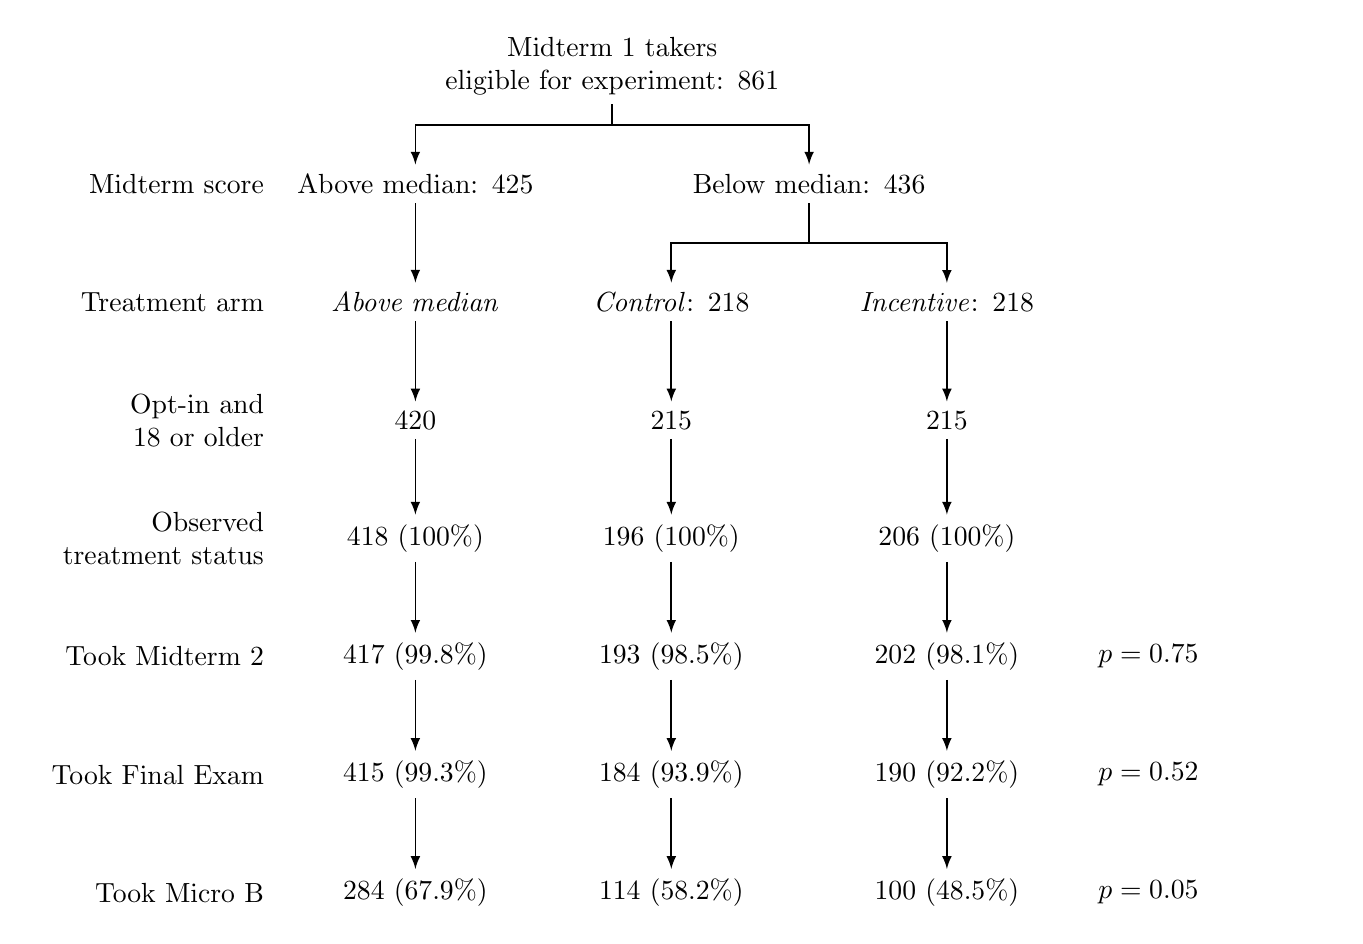
\begin{tikzpicture}[
	node distance=0mm,
	every node/.style = {shape=rectangle, draw=none, text width = 30mm, minimum height = 1em, align=center},
	pval/.style = {shape=rectangle, draw=none, inner sep=0mm, outer sep=0mm, minimum height=1em, align=left},
	cmnt/.style = {shape=rectangle, draw=none, inner sep=0mm, outer sep=0mm, minimum height=1em, align=right},
	level 1/.style = {sibling distance=50mm},
	level 2/.style = {sibling distance=35mm}, edge from parent fork down, edge from parent/.style = {draw, semithick, -latex},
	]
\begin{scope}
	\node [text width = 50mm] (L1) {Midterm 1 takers \\ eligible for experiment: 861}
		child {node (L2) {Above median: 425}
			child {node (L3) {\textit{Above median}}
				child {node (L4) {420}
					child {node (L45) {418 (100\%)}
						child {node (L5) {417 (99.8\%)}
							child {node (L6) {415 (99.3\%)}
								child {node (L7) {284 (67.9\%)}
								}}}}}}}
		child {node {Below median: 436}
			child {node {\textit{Control}: 218}
				child {node {215}
					child {node {196 (100\%)}
						child {node {193 (98.5\%)}
							child {node {184 (93.9\%)}
								child {node {114 (58.2\%)}
								}}}}}}
			child {node {\textit{Incentive}: 218}
				child {node (R4) {215}
					child {node (R45) {206 (100\%)}
						child {node (R5) {202 (98.1\%)}
							child {node (R6) {190 (92.2\%)}
								child {node (R7) {100 (48.5\%)}
								}}}}}}};
\end{scope}
% row labels, from bottom to top
\node[cmnt] (l7) [left=3mm of L7] {Took Micro B};
\node[cmnt] (l6) [left=3mm of L6] {Took Final Exam};
\node[cmnt] (l5) [left=3mm of L5] {Took Midterm 2};
\node[cmnt] (l45) [left=3mm of L45] {Observed \\ treatment status};
\node[cmnt] (l4) [left=3mm of L4] {Opt-in and \\ 18 or older};
\node[cmnt] (l3) [left=3mm of L3] {Treatment arm};
\node[cmnt] (l2) [left=of l3.east |- L2.west] {Midterm score};
%pvals, from top to bottom
\node[pval] (r5) [right=3mm of R5] {$p=0.75$};
\node[pval] (r6) [right=3mm of R6] {$p=0.52$};
\node[pval] (r7) [right=3mm of R7] {$p=0.05$};
\end{tikzpicture}
Percentages in parentheses are the portion of students who observe their treatment status and took the second midterm, final exam, and enrolled in Micro B, calculated separately for each treatment arm. The p-values are from a two-sample t-test of the equality of attrition rates between the \textit{Control} and \textit{Incentive} arms at each stage.
\end{center}
\end{figure}

Since all students below the median on the first midterm had equal probabilities of being assigned to the \textit{Control} and \textit{Incentive} arms, treatment arms are balanced on covariates in expectation. In practice, due to chance and nonrandom attrition, treatment arms can be unbalanced on covariates, which can bias estimates if not addressed in the analysis, particularly in small samples \parencite{ai2017}. We check balance on observable characteristics after attrition for both the second midterm and final exam samples. As can be seen in Appendix Tables \ref{balance_table_mid2} and \ref{balance_table_final}, we find no statistically significant difference between the \textit{Control} and \textit{Incentive} arms in observable covariates including first midterm score, year, previous term's cumulative GPA, videos watched before the first midterm, ethnicity, gender, and transfer status. However, as discussed in Section \ref{empiricalstrat}, to correct for potential imbalance and to improve precision, we estimate models that include controls chosen via the post-double-selection method of \textcite{bch2014a}.

\subsection{Relevancy of the encouragement instrument}

We use a Two-Stage Least Squares approach to estimate the LATE of watching videos on exam performance, as detailed in the Section \ref{empiricalstrat}. We must check that our instrument is both valid and relevant to ensure this method will produce an unbiased estimate of the LATE \parencite{ir2015}. The validity condition is met by assigning treatment at random conditional on midterm exam score and year of instruction. Balance across pretreatment observables, as demonstrated in Appendix Tables \ref{balance_table_mid2} and \ref{balance_table_final}, give us further confidence that treatment status is uncorrelated with demographics.

Next we check instrument relevancy, that is, whether treatment status generates significantly more video watching. In Table \ref{firststage_table} we present estimates from Equation \ref{itt_spec}. We find that by the second midterm exam, being assigned to the \textit{Incentive} arm induces students to watch 9.1 - 10.5 videos and 6.0 - 6.8 unique videos more than being assigned to the \textit{Control} arm. The gap between treatment and control grows by the final exam to 38.4 - 39.2 videos and 20.5 - 21.6 unique videos. The larger gap by the final is unsurprising given that the deadline to earn the grade incentive was the day before the final exam. Following the recommendations of \textcite{ass2019}, we assess the strength of our instrument using the effective F-statistic of \textcite{op2013} which, in our just-identified setting, coincides with the Wald statistic of \textcite{kp2006}. The effective F-statistic for the second midterm and final exam first-stage specifications are 18.6 and 194.6, respectively, both of which are greater than the \textcite{sy2005} critical value of 16.4 and the rule-of-thumb cutoff of 10.

Graphically, we depict the distribution of videos watched as a function of treatment in Figure \ref{combo_cdf}. Notably, the gap between treatment and control distributions remains significantly positive at every level of video watching by the final exam. The difference is most pronounced near the required number of videos to earn the grade incentive, after which the difference diminishes towards zero. For the second midterm sample, the difference is smaller but significantly different from zero between zero and 62 videos watched. We also show time series plots of video watching in Figure \ref{timeseries}, which show no differences in video watching before the first midterm and marked increases before the second midterm and final exam. Collectively, given the highly significant first stage regression results, large first-stage F-statistics, and monotonic increase in video watching across the sample, we have high confidence that our instrument meets the relevancy criterion.

%Zack--given the importance of bunching in the theory section, we need to add histograms (by treatment status and above median) of unique induced videos watched and total induced videos watched. We might also want to contrast with total videos watched across the three groups to show extnet of binge watching. Finally, this may be where we add which videos were watched more by the control group. Perhaps a new section called ``Video Watching Behavior: bunching, binging and the ``marginal" videos? This could also be the first part of the results section.

\subsection{Effects on exam scores}

In this section, we estimate the causal effects of being assigned to the \textit{Incentive} arm on exam scores (ITT). This estimate is relevant for educators interested in predicting how requiring videos will change exam scores in their classes using the same grade-based incentive implemented in our experiment. Additionally, we estimate the causal effect of watching videos on exam scores, which is of interest to educators deciding which teaching technologies to provide for their classes as well as to students choosing among different studying tools.

For both the ITTs and LATEs, we examine effects on the second midterm and final exams using both parametric methods (i.e. Equations \ref{itt_spec} and \ref{secondstage_spec}) and nonparametric methods a la the repeated sampling framework of \textcite{neyman1923}% and Generalized Random Forests proposed by \textcite{wa2018}
. We check that our parametric results are robust to model specification by estimating Equations \ref{itt_spec} and \ref{secondstage_spec} with and without $f(X_i)$ as a vector of linear control variables chosen via PDS \parencite{bch2014a}. To rule out nonrandom attrition across treatment arms as a confounder, we fit a fixed effect model that drops any student whose matched pair attrited. These specifications and identification strategies are described in detail in Section \ref{empiricalstrat}.

Table \ref{secondstage_table} presents estimates of the effects of treatment on second-midterm and final exam scores. Across our four specifications, we estimate reduced-form (RF) impacts of being assigned to the \textit{Incentive} arm of 0.17 - 0.18 standard deviations on the second midterm. These estimates, along with our first-stage estimates (Table \ref{firststage_table}), imply LATEs of 0.26 - 0.30 standard deviations per 10 unique videos, or 0.16 - 0.18 standard deviations per hour of unique content. For the final exam, we estimate similar ITT effects: being assigned to the \textit{Incentive} arm raises scores by 0.14 - 0.18 standard deviations. However, given the larger first stage effects for the final exam, we estimate smaller LATEs: 0.08 - 0.09 standard deviations per 10 unique videos, or 0.04 - 0.05 standard deviations per hour of unique content.

Given the large F-statistics when estimating first-stage effects of our incentive instrument on videos watched, we are not particularly concerned about bias from weak instruments. However, following the advice of \textcite{ass2019}, we report Anderson-Rubin confidence sets, which are efficient regardless of the strength of our instrument. As can be seen in Appendix Table \ref{arci_table}, we find that the weak-instrument-robust confidence intervals are very similar to those presented in Table \ref{secondstage_table}.

\subsection{Effects at the incentive cutoff}

Here we present estimates of treatment effects for students at the incentive-eligibility cutoff: the median score on the first midterm. While the primary intended purpose of cutoff was to avoid burdening high-performing students, the discontinuous change in treatment probability allows for identification of LATEs, as we describe in section \ref{empiricalstrat}. Unfortunately, the density of students at the cutoff is not enough to allow for precise identification of treatment effects. For completeness and bounding possible effect sizes, we share our findings.

Before using a regression discontinuity (RD) design in our setting, we must establish that students did manipulate their midterm scores to affect their chances of being treated. Intuitively, it would be surprising to find manipulation as students did not know the median score \textit{ex ante}. Additionally, it would be quite difficult to accurately predict one's midterm score while taking the exam, and those capable of doing so would likely have higher returns scoring higher than the median. Appendix Figure \ref{mid1dist} shows that, as expected, the distribution of midterm scores does not have any unordinary masses on one side of the cutoff.

In most RD designs, the researcher can only observe either treatment or control outcomes on one side of the cutoff. In our setting, however, we can observe control outcomes on \textit{both} sides of the cutoff. As such, we identify treatment effects adjusting the conventional RD approach to account for our increased knowledge of the control group's mean outcome at the cutoff. In practice, this entails differencing treatment and control conditional mean outcomes using local linear regressions where we calculate the control conditional mean using both \textit{Control} and \textit{Above median} observations.

Figures \ref{rdmid2} and \ref{rdfinal} in the Appendix depict the effects of treatment near the cutoff for the second midterm and final exams, respectively. Both Figures show a marked increase in video watching for treatment students at the cutoff. Both figures also show positive point estimates of the effect of treatment on exam scores for those at the cutoff, but neither of these point estimates are statistically distinguishable from zero. Appendix Table \ref{rdtable} summarizes the point estimates and confidence intervals for those at the incentive eligibility cutoff. We find that treatment increases video watching by 9.1 and 24.2 unique videos by the second midterm and final exams, respectively, and we find positive but not statistically significant effects on exam scores. The first-stage effects at the cutoff are in line with the estimated average first-stage effects for those below the median.

\subsection{Spillovers during concurrent term}

We next estimate spillover effects to other courses taken concurrently during the term of the experiment. Although we find positive effects on outcomes in Micro A, it is important to examine spillover effects to understand the complete picture of how treatment affects student achievement. If the gains in Micro A come at the cost of slowed progress in other courses, then treatment may be counterproductive for some students. On the other hand, since the videos cover concepts and methods that could be covered in other courses, treatment may help students outside Micro A.

Table \ref{spillover_grades} presents our estimates of Equation \ref{itt_spec} where $Y_i$ is GPA, number of classes passed, or portion of classes taken for a letter grade. We estimate the effects of treatment on term GPA calculated separately for all classes, all classes excluding Micro A, all classes outside of economics, and all economics classes excluding Micro A. In general, we find marginally significant or insignificant but directionally positive spillover effects on GPA.\footnote{At this university, term GPA is affected only by classes taken for a letter grade. Hence, students may not have attrited from the sample but may have taken all courses Pass/No Pass and thus have no term GPA. As such, we report sample sizes for each GPA specification.} We can rule out large negative spillover effects: in our worst-case specification for term GPA, our 95\% confidence interval rules out negative spillover effects larger than -0.02 (on a 4.0 scale), or less than 1\% of the mean term GPA among control students. There is no statistically significant difference between our estimates of spillover effects on GPA when restricting to only economics or non-economics courses.

We additionally estimate the effects of treatment on number of classes passed and find small, insignificant, but directionally positive effects. We find that treatment caused students to pass 0.02 - 0.09 more classes, or about 1\% - 3\% more classes than the control mean. We find no effect of treatment on number of classes not passed or withdrawn. Interestingly, treatment students were somewhat less likely to take Micro A for a letter grade than were control students, but this difference is only marginally significant for one of the four specifications and insignificant for the rest. We find no relationship between treatment and fraction of classes taken for a letter grade versus Pass/No Pass. Across all grade spillovers examined, we find mostly small, directionally positive effects, which gives us confidence that treatment is likely not harmful to academic success outside of Micro A.

Besides estimating spillover effects on other course grades, we also examine spillovers to other studying methods within Micro A. Doing so helps us better understand mechanisms: do students substitute away from other studying when encouraged to watch more videos, or are they more likely to complement their video-watching with other unincentivized studying? In Table \ref{spillover_studying}, we display the results of estimating equation \ref{itt_spec} where $Y_i$ is an alternative form of studying. We find that \textit{Incentive} students are directionally less likely to attend class, though not statistically significantly so. On the other hand, treatment students interacted with the online discussion board more than did control students, but again these estimates are not statistically distinguishable from zero. We do not find any significant relationship between treatment and tutoring attendance.

\subsection{Spillovers to subsequent term}

While we offered treatment students a grade incentive to watch videos during Micro A, students were not offered a grade incentive during the subsequent course in the intermediate microeconomics sequence, Micro B. However, all students in Micro B maintained access to the IMVH and were verbally encouraged to watch videos as a study method. Fortunately, we are able to observe video watching and grade outcomes in Micro B.

We present our estimates of spillover effects during the subsequent term in Table \ref{spillover_100b}. In Panel A, we estimate the effect of treatment on videos watched during the subsequent term, for those who took Micro B. We find large and statistically significant effects: treatment caused students to watch 8.1 - 9.9 more unique videos and 1.2 - 1.5 hours of unique content compared to control students. In Panel B, we estimate equation \ref{itt_spec} where $Y_i$ is the first midterm, second midterm, or final exam score. Unfortunately given the small subsample of students who took Micro B, we are underpowered to detect effect sizes consistent with those observed during Micro A. Finally, in Panel C, we estimate the effect of treatment on taking Micro B and the number of classes passed and withdrawn. We find no effects statistically distinguishable from zero, though, as mentioned in section \ref{attrition}, treatment students were directionally less likely to take Micro B than were control students.

\section{Models of Studying Behavior} \label{models}

To understand our empirical results in the context of economic theory, we discuss three models of student studying behavior: a neoclassical model, an imperfect information model, and a behavioral/ procrastination model. For each model we consider the testable implications of a grade inducement to encourage adoption of a study method.\footnote{For all three models, we do not address the issue that the IMVH is a relatively unique study tool in that, to our knowledge, it is the first instructional book to be created entirely of videos. However, given the availability of close substitutes to the IMVH (lecture capture, for example) we do not explore the added issues of inducing students to use a study tool whose usefulness is not known to the instructor.} Neoclassical models of studying behavior assume that rational agents know their returns to studying using the methods available to them and allocate the optimal study time to each method given their utility function, which is increasing in leisure and grades and decreasing in time spent studying. College instructors have little knowledge about student utility functions and do not know student preferences over performance in other classes or other uses of the student's time which may also have large payoffs in the labor or marriage markets. In this model, there is no room for an instructor to increase student well-being by intervening in their study decisions. Both \textcite{oettinger2002} and \textcite{kow2020} find empirical support for the neoclassical model. \textcite{oettinger2002} finds that student effort responds rationally to nonlinear grade incentives: across 1200 students in a principles of economics class with absolute grading standards, he finds evidence of bunching just above letter grade cutoffs and student performance on the final exam is higher if the student is just below a grade threshold. \textcite{kow2020} explore the effects of a university policy that required students who performed poorly in their first year to attend a large fraction of the tutorials for each class in their second year. At the poor performance threshold, both tutorial and lecture attendance increased by over 50 percent with a concomitant decline in self-study hours. Grades for students at the policy threshold were \textit{lower} by 0.16-0.26 standard deviations. At least for students at the margin of poor performance, the requirement to attend tutorials appears to have hurt students by not allowing them to pick their optimal study strategy across self-study, turorials and lectures.

A key assumption of the neoclassical model is that students possess complete information about the returns across studying methods. However, there is evidence from psychology that college students do not know the return to various study options\footnote{See, for example, \textcite{mccabe2011}, \textcite{prcc2007}, and \textcite{drmnw2013}} and many universities fund ``Teaching and Learning Centers" or ``Academic Skills Centers," part of whose mission is to help undergraduates learn to study more productively.\footnote{All nine University of California campuses have such a center. Examples outside the UC include Dartmouth's Academic Skills Center, Michigan's Center for Research on Teaching and Learning, UNC's Learning Center, and Yale's Teaching and Learning Center.} Further, the ``raison d'etre" of higher education is not only to teach students specific skills but to teach students how to learn. As an alternative to the neoclassical model, we hypothesize that students supply a quantity of study time that is optimal given their information constraints. In this `imperfect information' model, students choose study methods and quantities that are suboptimal relative to those they would have picked in a full information setting. Hence, an intervention by an entity that has more information about returns to studying across various methods (i.e. an instructor) can enhance student utility.

A third model is a behavioral one in which students plan to study more than they end up studying when the time comes. This phenomenon is consistent with two-self models in which a person's ``planner" self, the one who desires high grades at the expense of leisure, is at odds with her ``doer" self who must choose between immediately gratifying leisure and delayed gratification from higher grades. Indeed, survey and experimental data suggest that many students study less than they report they ``should" and finish the term with grades lower than what they had anticipated they would earn at the start of the term.\footnote{See, for example, \textcite{ferrari1992}, \textcite{ccog2017} and \textcite{lo2016}.} \textcite{cgpr2020} provide empirical support for this model by finding that setting tasked-based goals helps improve college student performance. As descriptive evidence in support of this model, \textcite{blmo2019} find that students that do much worse than expected in college are those who say they have poor time management or procrastination issues, including a tendency to cram and spending very little time studying.

We consider the testable implications of the three models applied to a setting where students are incentivized to use a time-consuming educational input, say, a set of instructional videos (or attending class, reading the textbook, working on homework, etc.). The incentive is structured such that students who consume the educational input receive a higher grade in the course by consuming a set level of the input. In this simple setting, students gain utility only from leisure and grades. We assume grades, a function of time spent studying, and utility are both continuous, smooth, and increasing and concave in their inputs. Students can choose to study using the incentivized educational input, $v$, or some outside option that is not directly incentivized, $o$, or a combination thereof.

Across all three models, before the first educational input is incentivized, students allocate time to the two studying methods until the marginal benefit of each (through higher grades) is equal to the marginal cost of forgone leisure. Consider the population of students initially consuming below the requisite level to earn the grade incentive. These students must decide if earning the grade incentive is worth forgone leisure and less time allocated to their outside studying option. Next we explore the differences in predictions across the three models.

% For the `compliers' - those for whom the incentive induces greater take-up of the incentivized input -

% Depending on the relative returns to studying and the students' preferences, it is theoretically ambiguous how adding the incentive will affect grades. Next we highlight the primary differences between the models.

% Do we want to write formal models? I think we should...it may be easier for some to see the implications if presented as equations.

\begin{figure}
	\begin{center}
		\begin{tikzpicture}[scale=0.6]
			% axes
			\draw [thick,<->] (0,8) node[left]{$v^*(L)$}--(0,0)--(11,0) node[right]{$L$};
			\node [below left] at (0,0) {$0$};

			% v*
			\draw (0,5) -- (2,4);
			\draw (2,4) -- (6,4);
			\draw (6,4) -- (6,2);
			\draw (6,2) -- (10,0);
			\draw [dashed] (2,4) -- (6,2);

			% video incentive threshold
			\node [left] at (0,4) {$T$};
			\draw (-0.1,4) -- (0.1, 4);
			\node [below] at (6,0) {$1-T$};
			\draw (6,-0.1) -- (6,0.1);
			%\draw [dashed] (0,4) -- (10,4);
			%\draw [dashed] (6,0) -- (6,10);

			% points for U1 and U2
			\draw [fill] (4.4,2.8) circle [radius=.05];
			\node [below] at (4.4,2.8) {$v_1$};
			\draw [fill] (3.95,4) circle [radius=.05];
			\node [above] at (3.95, 4) {$v_2$};

		\end{tikzpicture}

		\vspace{1\baselineskip}

		% Utility curves
		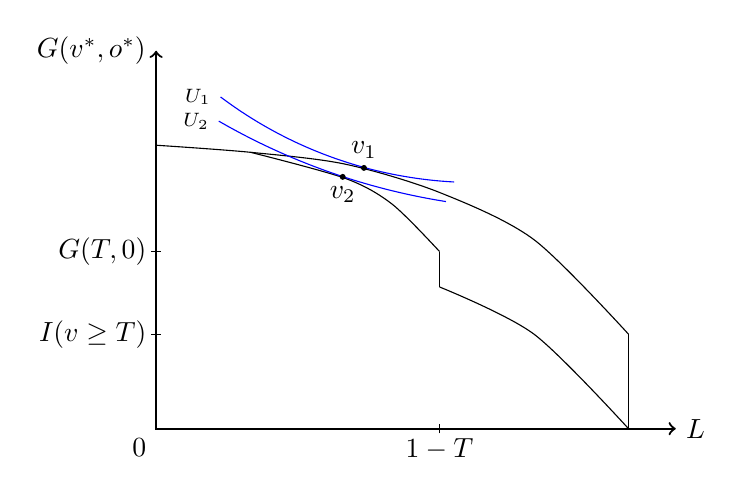
\begin{tikzpicture}[scale=0.6]
			% axis
			\draw[thick,<->] (0,8) node[left]{$G(v^*,o^*)$}--(0,0)--(11,0) node[right]{$L$};
			\node [below left] at (0,0) {$0$};
			% video incentive threshold
			\node [below] at (6,0) {$1-T$};
			\draw (6,-0.1) -- (6,0.1);

			% production frontier 1 - not incentivized
			\draw (10,0)--(10,2);
			\draw plot [smooth] coordinates {(10,2) (8,4) (6,5) (4,5.6) (2,5.85) (0,6)};

			% production frontier 2 - incentivized
			\draw plot [smooth] coordinates {(10,0) (8,2) (6,3)};
			\draw (6,3)--(6,3.75);
			\draw plot [smooth] coordinates {(6,3.75) (5,4.75) (4,5.3) (2,5.85)};

			% indifference curves
			% original
			\draw[blue] (4,5.65) arc[start angle=252, delta angle=15, radius=9cm];
			\draw[blue] (4,5.65) arc[start angle=252, delta angle=-19, radius=9cm] coordinate (u1);
			\node[left] at (u1) {\scriptsize $U_1$};
			% tangency
			\draw [fill] (4.4,5.52) circle [radius=.05];
			\node [above] at (4.4,5.52) {$v_1$};

			% new
			\draw[blue] (4,5.32) arc[start angle=252, delta angle=9, radius=14cm];
			\draw[blue] (4,5.32) arc[start angle=252, delta angle=-12, radius=14cm] coordinate (u2);
			\node[left] at (u2) {\scriptsize $U_2$};
			% tangency
			\draw [fill] (3.95,5.33) circle [radius=.05];
			\node [below] at (3.95, 5.33) {$v_2$};

			% grade incentive
			\node [left] at (0,3.75) {$G(T,0)$};
			\draw (-0.1,3.75) -- (0.1,3.75);
			\node [left] at (0,2) {$I(v \geq T)$};
			\draw (-0.1,2) -- (0.1,2);


		\end{tikzpicture}

		\caption{A student maximizes her utility $U$, a function of leisure hours, $L$, and grades, $G$. Grades are a function of video watching hours, $v$, and hours spent on the next best studying option, $o$. \textit{Above}: Let $v^*(L)$ be the demand curve for video watching as a function of leisure $L \in [0,1]$. Assume the student maximizes her utility by watching $v_1$ videos and spending $o_1$ hours on her other study method. Suppose an instructor offers a grade incentive worth $I$ units, which a student can earn by watching $v \geq T$ hours of videos. At $L=1-T$ hours of leisure, the student maximizes grades by spending all study time watching videos, that is, $v^*=T$.
		\textit{Below}: Student's utility maximization problem for the neoclassical model. The grade incentive, $I$, is given to the student conditional on watching $T$ hours of videos (inner budget constraint) or, in the unincentivized case, given regardless of video watching (outer budget constraint). Time bundles along the inner budget constraint are weakly less prefered since the incentive draws the student away from otherwise more efficient $(v,o)$ combinations.}
	\end{center}
\end{figure}

In the neoclassical model, as long as $o$ and $v$ are not perfect , the marginal return to grades of the incentivized input is less than that of the outside option for the `compliers', or those induced by the incentive to consume at least a fixed level of the incentivized input. This model predicts bunching at the incentivized level cutoff since compliers would prefer to spend their marginal hours on leisure or studying with their other method. This model predicts a strict increase in video watching and weak decrease in other studying and leisure consumption. It is ambiguous whether cumulative study time increases or decreases as this depends on relative utility benefits of leisure and grades and the returns to studying by each method. However, if cumulative study time remains constant or decreases, then exam performance should strictly decrease since students are now suboptimally allocating study time versus their first-best allocation when considering only marginal returns to studying. On the other hand, if cumulative study time increases, students may earn greater exam grades but achieve lower utility compared to baseline. Importantly, this model predicts that in subsequent quarters students return to their pre-incentive levels of studying.

In the imperfect information model, students' \textit{ex ante} allocations to each studying method are not necessarily first-best. Compliers update their priors about the returns to watching videos as they work towards hitting the minimum required level for the grade incentive. At this cutoff, they make a decision whether to continue watching videos depending on their updated perceptions of the marginal benefit. We do not expect bunching in this model unless students believe the cutoff for the grade incentive is the optimal level or the updated marginal benefit at the cutoff is lower than the marginal benefit of the next best studying option or the marginal utility of leisure. A sharp prediction is that video watching will continue at the incentivized level in the absence of the grade incentive as students have learned an effective study tool. We also expect the treatment effect to be greater for students with more information problems, perhaps students in their first semester/quarter at university.

Finally, in the behavioral model, the instructor's inducement helps students stick to study plans up to the minimum required level for the grade incentive. As long as total study time does not fall, the inducement will increase exam performance. This model also predicts bunching at the incentivized level cutoff as long as using the incentivized input does not change the student's ``planner" and ``doer" selves. In the absence of the inducement, i.e., in future classes, a sharp prediction is that video watching will revert to pre-inducement levels.

One key empirical difference across the models is whether or not students return to their pre-incentive level of video watching in the absense of the incentive. We find that treated students continued watching videos in the absence of any grade incentive in Micro B, which is inconsistent with the predictions from both the neoclassical and behavioral models of learning in our setting. Another key empirical difference across the models is whether students watch exactly 40 videos, the number of videos rquired to earn the grade incentive. Both the neoclassical and behavioral models predict bunching at 40 videos and we find that treated students typically watched more 40 videos and do not find evidence of bunching. Since it was not easy for students to keep track of the videos they watched, the lack of bunching may simply reflect student uncertainty about whether they had met the 40-video threshold. Nevertheless, we view our results as most consistent with the imperfect information model of learning.

 % TODO non native English speakers or non citizenst


% *****************************************************************
% Discussion
% *****************************************************************

\section{Discussion} \label{discussion}

Here we discuss the findings reported in Section \ref{results}.

Contributions: First, we find that a small grade incentive is effective in motivating poorly performing college students to take-up video watching. We also reduced the weight on an early assessment and allowed students to earn back the lost points fully by meeting the video watching requirement, which may also be an important motivator. This result adds to the literature on what motivates college students to use educational inputs including financial incentives (see papers cited in \textcite{gmr2011}), requiring students to attend class if they perform poorly on an early assessment but with no penalty for not attending (as in \textcite{dgm2010}, or by having students set goals on the use of an practice quizzes and, again, no penalty, for failing to achieve the goal \parencite{cgpr2020}.\footnote{Note, in contrast to \textcite{cgpr2020}, \textcite{oppp2019} find that setting a weekly schedule ahead of time and weekly reminders via a text message had only a small effect on study time and no effect on output as measured by grades, retention or credit accumulation. In contrast to the effectiveness of incentives on college student use of educational inputs, several papers find incentives to directly increase output, such as grades or performance on exams, are less effective. See for example, \textcite{fryer2011} shows that paying students in K-12 to increase inputs shows greater effects than paying for increased output, \textcite{gmr2011} also point out that incentives in education appear to work better for inputs than output} Grade incentives have the unappealing feature that grades are directly a function of input use. The grade incentive used in this study was small, at most four percent of the student's grade, which may help mitigate this concern.

Second, we find that inducing students who performed poorly on an early assessment to increase the amount of time they spend watching instructional videos increased their exam performance. Since there was no drop in either grades for other courses taken in the same quarter or a drop in the use of many other educational for the class, this suggests that total study time for the course increased for treated students. Unfortunately, we were not able to determine where the added study time for the course did come from, which is important for student welfare calculations. Our results are consistent with other experimental and quasi-experimental studies that find positive effects of educational inputs on college student performance. %Zack--we need to contrast our results with other studies to see which input appears to most effective at increasing performance. See the ClarkGillProwseRush paper, section on benchmarking.

Third, while not statistically significant, it seems worth pointing out that we found positive point estimates on treated student's use of other educational inputs (attending class, downloading material from the course web page, and attending a tutoring lab) and grades in other courses taken in the same quarter compared to the control group. This surprising result was also found by \textcite{dgm2010} who required poorly performing students to attend class. The authors posit that the statistically insignificant but positive spillovers they find may be due to fixed effects of coming to campus. A fixed effects argument is less compelling in our context.

Finally, we find support for an imperfect information model of learning because treated students frequently watched more than the 40 videos they were required to watch to get the grade incentive and because treated students continued watching videos at a significantly higher rate in the following class when videos were not incentivized. \textcite{alo2009} also find continued higher use of academic support services after the incentivized year for women. An imperfect information model of learning can also account for why incentivizing educational inputs has been found to be more effective than incentivizing grades or exam performance directly (see studies cited in \textcite{gmr2011})

\textcite{aws2015} review the literature on using technology to provide supplemental aids for students in traditional classrooms and conclude that there is little causal evidence that student achievement is improved. The current study stands in contrast to this prior literature. In particular, they conclude that online instruction appears to have a negative effect on course grades and persistence. A more recent paper by \textcite{bflt2017} confirms these results, particularly for low performing students. The IMVH is clearly the backbone for an online class as it includes all the videos one would require students to watch as part of an online course. Perhaps the main effect of the video-watching requirement in this study was to increase student study time. Would encouraging at-risk students to watch instructional videos in an online class be as effective as we find for a in-person class? We consider this an important area for future research.

\subsubsection{Experiment design choices and \textit{local} treatment effects}

Our experiment contains several cutoffs: a midterm score cutoff below which students are eligible for the experiment, a video cutoff above which treatment students earn the grade incentive, and a date after which videos no longer count towards the incentive. All of these cutoffs influence the treatment effect estimates, which are \textit{local} to compliers. Specifically, we estimate the effect of videos for those induced by the incentive to watch, so changing who is induced and the videos they are induced to watch will affect estimates of the LATE. Though the purpose of this study was not to identify optimal thresholds, we discuss some observations that may motivate future work and explain our intuition for the size of the \textit{population} average treatment effect (ATE).

We required treatment students to watch 40 of 48 eligible videos to receive the incentive, giving students some agency in which videos they chose to watch. To better understand how the composition of watched videos differs between treatment arms, we plot video watch rates by video in Figure \ref{video_cdf}. This plot reveals that the videos students chose to watch are not random. Watch rates in the control group vary across videos from nearly 0\% up to over 70\%, demonstrating that the perceived intrinsic value of videos varies considerably. For treatment students, watch rates vary less across videos but are positively correlated with control watch rates. Notably, treatment watch rates are 70\% or greater for videos whose control watch rates are between 5\% and 20\%. This gap has implications for the estimated local average treatment effect: if treatment encourages students to watch low value videos, then the LATE estimate will be diluted relative to the population ATE.

We investigate this gap first by considering whether treatment encouraged students to watch shorter videos. One may hypothesize that treatment students would choose to skip the longest videos since earning the incentive is not dependent on length of videos. If students picked the shortest 40 videos, they would watch 1.6 fewer hours of content versus watching the longest 40 videos. We fit a linear model that predicts a video's treatment watch rate using the duration of the video and its control watch rate.\footnote{It is important to control for the control group's watch rate since the educational value of a video may be endogenously related to its length (e.g., harder concepts take longer to explain).} Using this model, we find that each additional minute in duration is associated with a 0.3 percentage point decrease in watch rate by the treatment group. For the longest incentivized video, this corresponds with a predicted 3.7 percentage point lower watch rate compared to the average length video. We interpret this finding, given the strong correlation between control and treatment watch rates, as evidence that \textit{content} is a more important driver than is minimizing time cost when choosing which videos to watch. However, it is plausible that some students prioritized shorter-length videos.

Next, we examine how watch rates varied over time. In Figure \ref{video_cdf_week} we plot watch rates by video organized by week each video's content was covered in class. Interestingly, control group watch rates taper off towards the end of the term while treatment watch rates remain much higher. This observation is consistent with the video incentive serving as a commitment mechanism, perhaps encouraging students to spend more time stuyding for the final exam. Alternatively, perhaps control students watch fewer videos in weeks nine and ten as they shift their study time to other methods while preparing for the final. It is theoretically ambiguous whether the gap in watch rates towards the end of the term suggests a larger or smaller LATE relative to the population ATE.

Finally, we consider the influence of the due date on our treatment effect estimates. To earn the grade incentive, students had to watch 40 videos by the last day of instruction, which is the day before the final exam. This is an intuitive deadline, but it allows procrastination-prone students to delay watching many hours of videos until the final week of the term. It is plausible that these students could be harmed by treatment, or at the very least have very small treatment effects, which could explain part of the reason why our LATE estimates are smaller for the final exam than the second midterm. To get a sense of whether treatment students were more likely to ``binge watch" videos, we plot the max number of videos watched in one week per student in Figure \ref{hist_binge}. Though some control students watch 40 or more videos in one week, this behavior seems more prevalent in the treatment group. While this may very well be a useful, rational studying strategy for some, research suggests that spreading learning over time may be more effective \parencite{kornell2009}. \textcite{aw2002} find that offering deadlines, though costly from a rational agent perspective, results in better grades. As an alternative to one deadline, offering multiple deadlines, perhaps weekly or shortly before both exams, may improve consistency between treatment effect estimates for the two exams.

Collectively, it is not obvious how the population ATE compares with the LATEs we estimate. Neoclassical economic theory suggests that those who select into watching videos regardless of exogenous incentives likely do so because they benefit more than those who only select into watching videos only in the presence of exogenous incentives. This view would suggest that the population ATE is greater than the LATE. However, this view is, perhaps, inconsistent with the alternative that students may not how much studying is optimal, or what they should be studying. While it is not possible to estimate the population ATE given our experimental design, our intuition is that the ATE is likely higher than the LATE estimated for the final exam and closer to that estimated for the second midterm, which is less likely to be diluted from deadline-induced binge watching and selecting the shortest videos.

\subsection{Limitations}

The present study has several limitations that should be considered before, for example, creating one's own video handbook and requiring students to use it. First, the population studied is students who score below the median on the first midterm of an intermediate microeconomics course at a large, highly-selective public research university. The extent to which treatment effects vary by course, instructor, university, or along the top half of the midterm score distribution is important but beyond the scope of this paper.\footnote{\textcite{ck2020} is an example where an intervention that was effective in raising exams scores in introductory microeconomics classes at large public research university but did not raise exam scores across several different types of classes in a broader-access institution.} Additionally, the causal effects of watching videos that we estimate are \textit{local} to compliers, i.e. students induced by the grade incentive to watch additional videos. We cannot recover the \textit{population} average treatment effect, though anecdotal evidence and economic theory both suggest that the population average treatment effect is likely greater than the LATE because control students watched many videos even without incentive

Universities often have policies that emphasize improving the performance poorly performing students, such as academic probation policies and the policy studied by \textcite{kow2020}. We focus on students who perform poorly on the first midterm, a population simliar to that of \textcite{dgm2010}. However, some researchers may ponder why we elected to include only the bottom half of the first midterm distribution in the experiment rather than the entire class. While including the entire class would have increased statistical power, we believe the additional precision might have come at the expense of welfare losses by high performing students. The first midterm provides a signal of which students likely know for themselves how to study, both methods and duration. Coercing these high-type students to spend time with a potentially different studying method runs a greater risk of harming utility. On the other hand, students who, through a low midterm score, make manifest a need for alternative studying practices stand to benefit the most from instructor-provided guidance.

The positive effects we estimate are attributable to watching IMVH videos and, perhaps, spending a greater amount of time studying for the course in general. Our experimental design does not allow us to separately identify the effects of these two mechanisms for improving exam performance. Would a similar incentive structure that induces greater takeup of an alternative studying method have similar effects? We view this as an important question for future research. While all studying methods require time, some are more efficient than others in terms of effects per unit time. Besides time, learning tools often carry additional costs that should be taken into consideration. For example, students must often purchase textbooks for courses that require textbooks, which may disadvantage students from low-resourced families. Some tools can add costs to the instructional team who, for example, must create and grade problem sets. Internet-delivered videos have the advantage of near-zero marginal financial cost to students and zero marginal time or financial cost to the instructional team.

Another consideration is the time frame during which the experiment took place, 2018 to 2019. About three months after the conclusion of our experiment, most students in the United States and all students at the studied university began remote learning as the COVID-19 pandemic prompted stay-at-home orders. With increased experience learning via electronic media, it is possible that treatment effects will be higher in the future than we estimate in our paper. On the other hand, if students find online learning materials increasingly \textit{less} engaging, we may find the opposite.

In addition to estimating the effects of video handbooks in other educational settings, future research should examine treatment effects in the presence of weekly deadlines instead of one final deadline at the end of the term. Given our observation of greater ``binge watching" by treatment students and the smaller effect sizes before the final exam compared to the second midterm exam, we suspect weekly deadlines may reduce the deleterious effects of procrastination. Despite the rich literature on the advantages of spread-out studying \parencite{kornell2009, cpvw2006}, we note that ``binge watching" was not unique among treatment students. Indeed, most students within each treatment arm watched more videos the last week of the term than any other week.

% *****************************************************************
% Conclusion
% *****************************************************************

\section{Conclusion} \label{conclusion}

We examine the effectiveness of an innovative educational technology, a video handbook composed of 220 brief instructional videos on intermediate microeconomic theory. We used random assignment of a grade-based incentive to experimentally vary takeup of the video handbook, and we found that greater takeup caused student to score significantly higher on exams. Specifically, we estimate that treatment causes students to score about 0.18 standard deviations higher on midterm and final exams. For students on the margin of watching videos, watching an additional hour of unique content causes students to score between 0.05 to 0.15 standard deviations higher on exams.

Instructors may have concerns about making a resource such as the IMVH available if they believe students may substitute away from lectures or other more productive studying methods \textcite{kay2012}. Another concern is that forcing students to spend more time studying in one's class may worsen performance in other classes. Our analysis provides some confidence that neither of these fears are first-order concerns. We do not find evidence that students decrease their consumption of other forms of studying, nor do we find that students perform worse in other courses during the same quarter. Our point estimates of the effect of treatment on takeup of other studying methods, though not statistically significantly different from zero, are \textit{positive} for most alternatives, suggesting that if any, students consider the videos complements to other forms of studying. A potential mechanism might be that the videos help students realize what they \textit{don't} know, increasing the marginal benefit of subsequent studying.

A final concern is one of welfare. In a neoclassical model, instructors cannot make their students better off by exogenously incentivizing quantities of studying they would not otherwise have chosen for themselves. In an imperfect information model, which we think is more appropriate in our university classroom setting, instructors \textit{can} improve student welfare through intervention when information barriers lead to suboptimal time allocation decisions. We observe two phenomena that support this model. First, treated students do not bunch at the cutoff for the grade incentive. Second, video consumption remains much higher among treated students in the term following conclusion of the experiment.

While there are many educational interventions that instructors could offer their students, the research on causal effects of educational interventions remains limited. Our study serves as an example of a feasible research design that runs a lower risk of generating welfare losses for high performing students than does a class-wide experiment. It is our hope, as educators ourselves, that more research be conducted on the effectiveness of pedagogical technologies.

\printbibliography

%%% TABLES

\clearpage
\begin{spacing}{1.0} 
\begin{table} \centering \caption{Effects of Grade Incentive on Video Watching} 
\label{firststage_table} 
\begin{threeparttable} 
\begin{tabular}{m{0.35\linewidth} *{5}{>{\centering\arraybackslash}m{0.1\linewidth}}}
\toprule
                               & Control Mean &       (1) &       (2) &       (3) &       (4) \\
\midrule
                        
\multicolumn{6}{l}{\textbf{Panel A}: By Midterm 2} \\ 

\customlinespace \indentrow{Videos} &        33.91 &  10.19\sym{***} &  10.54\sym{***} &   9.08\sym{***} &   9.58\sym{***} \\
                               &              &    (2.85) &    (3.12) &    (2.03) &    (2.19) \\
                 
\customlinespace \indentrow{Unique videos} &        23.13 &   6.63\sym{***} &   6.79\sym{***} &   5.97\sym{***} &   6.11\sym{***} \\
                               &              &    (1.54) &    (1.70) &    (0.98) &    (1.11) \\
               
\customlinespace \indentrow{Hours of videos} &         5.88 &   1.68\sym{***} &   1.72\sym{***} &   1.48\sym{***} &   1.55\sym{***} \\
                               &              &    (0.50) &    (0.55) &    (0.35) &    (0.38) \\
        
\customlinespace \indentrow{Hours of unique videos} &         3.85 &   1.10\sym{***} &   1.13\sym{***} &   0.99\sym{***} &   1.02\sym{***} \\
                               &              &    (0.25) &    (0.28) &    (0.16) &    (0.18) \\
                  
\midrule 
Observations &              &       395 &       362 &       395 &       362 \\
                        
\midrule 
\multicolumn{6}{l}{\textbf{Panel B}: By Final Exam} \\ 

\customlinespace \indentrow{Videos} &        53.09 &  39.25\sym{***} &  39.07\sym{***} &  38.57\sym{***} &  37.99\sym{***} \\
                               &              &    (4.06) &    (4.37) &    (3.40) &    (3.69) \\
                 
\customlinespace \indentrow{Unique videos} &        33.95 &  21.55\sym{***} &  21.08\sym{***} &  21.28\sym{***} &  20.49\sym{***} \\
                               &              &    (1.55) &    (1.66) &    (1.22) &    (1.27) \\
               
\customlinespace \indentrow{Hours of videos} &         8.93 &   6.30\sym{***} &   6.26\sym{***} &   6.18\sym{***} &   6.05\sym{***} \\
                               &              &    (0.69) &    (0.75) &    (0.57) &    (0.62) \\
        
\customlinespace \indentrow{Hours of unique videos} &         5.54 &   3.43\sym{***} &   3.36\sym{***} &   3.38\sym{***} &   3.26\sym{***} \\
                               &              &    (0.25) &    (0.27) &    (0.20) &    (0.21) \\
                  
\midrule 
Observations &              &       374 &       332 &       374 &       332 \\
 Treatment assignment controls &              &       Yes &        No &       Yes &       Yes \\
          Demographic controls &              &        No &        No &       Yes &       Yes \\
            Pair Fixed Effects &              &        No &        No &        No &       Yes \\
\bottomrule
\end{tabular}
\Fignote{Model (1) contains linear controls for midterm 1 score and year; (2) is the difference in means and standard errors calculated using the repeated sampling framework of Neyman (1923); (3) and (4) use the post-double-selection (PDS) procedure of \textcite{bch2014a} to select control variables then estimate treatment effects and standard errors. The control variables selected using PDS are listed in Table \ref{controlvars_selected_itt}. Models (2) and (4) include only students whose matched-pair did not attrite from the experiment. \textit{Control Mean} is the mean for the Control students included in models (1) and (3), which is nearly identical to the mean for the Control students included in models (2) and (4). \Regnote} 
\end{threeparttable}
\end{table} 
\end{spacing}

\clearpage
\begin{spacing}{1.0} 
 \def\sym#1{\ifmmode^{#1}\else\(^{#1}\)\fi} 
\begin{table} \centering \label{secondstage_table} 
 \caption{Effect of Videos on Grades} 
\begin{threeparttable} 
\begin{tabular}{m{0.35\linewidth} *{4}{>{\centering\arraybackslash}m{0.1\linewidth}}}
\toprule
                                     &      (1) &      (2) &      (3) &      (4) \\
\midrule
          \multicolumn{5}{l}{\textbf{Panel A}: Midterm 2 Score} \\ 
\indentrow{RF: Incentive}  &    0.18\sym{*} &    0.18\sym{*} &    0.18\sym{*} &    0.17\sym{*} \\
                                     &  (0.090) &  (0.094) &  (0.090) &  (0.096) \\
        \customlinespace \indentrow{2SLS: 10 Videos}  &   0.027\sym{*} &   0.027\sym{*} &   0.030\sym{*} &   0.029\sym{*} \\
                                     &  (0.015) &  (0.015) &  (0.015) &  (0.015) \\
 \customlinespace \indentrow{2SLS: 1 Hour of Videos}  &   0.224\sym{*} &   0.233\sym{*} &  0.238\sym{**} &   0.222\sym{*} \\
                                     &  (0.128) &  (0.138) &  (0.121) &  (0.124) \\
                        \customlinespace Observations &      395 &      362 &      395 &      362 \\
          \midrule 
 \multicolumn{5}{l}{\textbf{Panel B}: Final Exam Score} \\ 
\indentrow{RF: Incentive}  &   0.17\sym{**} &    0.17\sym{*} &   0.17\sym{**} &     0.14 \\
                                     &  (0.089) &  (0.103) &  (0.088) &  (0.103) \\
        \customlinespace \indentrow{2SLS: 10 Videos}  &  0.008\sym{**} &   0.008\sym{*} &  0.008\sym{**} &   0.009\sym{*} \\
                                     &  (0.004) &  (0.005) &  (0.004) &  (0.005) \\
 \customlinespace \indentrow{2SLS: 1 Hour of Videos}  &  0.074\sym{**} &   0.074\sym{*} &  0.074\sym{**} &    0.058 \\
                                     &  (0.038) &  (0.045) &  (0.037) &  (0.044) \\
                        \customlinespace Observations &      374 &      332 &      374 &      332 \\
       \midrule 
 Treatment assignment controls &      Yes &       No &      Yes &      Yes \\
                Demographic controls &       No &       No &      Yes &      Yes \\
                  Pair Fixed Effects &       No &       No &       No &      Yes \\
\bottomrule
\end{tabular}
\Fignote{This table reports coefficients on $Incentive_i$ from Equation \ref{late_spec} and $Video_i$ from Equation TBD. Test scores are measured in standard deviation units. Model (1) contains linear controls midterm 1 score and year; (2) is the difference in means and standard errors calculated using the repeated sampling framework of Neyman (1923); (3) and (4) use the post-double-selection (PDS) procedure of \textcite{bch2014a} to select control variables then estimate treatment effects and standard errors. The control variables selected using PDS are listed in Table \ref{controlvars_selected_itt}. Models (2) and (4) contain only students whose matched-pair did not attrite from the experiment.  \Regnote} 
 \end{threeparttable} 
 \end{table} 
 \end{spacing}

\clearpage
\begin{spacing}{1.0} 
\begin{table} \centering \caption{Spillover Effects of Incentive on Other Course Grades} 
\label{spillover_grades} 
\resizebox{0.9\linewidth}{!}{% 
\begin{threeparttable} 
\begin{tabular}{m{0.35\linewidth} *{5}{>{\centering\arraybackslash}m{0.1\linewidth}}}
\toprule
                               & Control Mean &     (1) &     (2) &     (3) &     (4) \\
\midrule
                   
\multicolumn{6}{l}{\textbf{Panel A}: Effects on Term GPA} \\ 

\customlinespace \indentrow{All classes} &         2.59 &  0.13\sym{**} &   0.13\sym{*} &   0.11\sym{*} &    0.10 \\
                               &              &  (0.06) &  (0.07) &  (0.06) &  (0.06) \\
                   &              &     373 &     332 &     373 &     332 \\
             
\customlinespace \indentrow{Excluding Micro A} &         2.75 &    0.10 &    0.11 &    0.09 &    0.10 \\
                               &              &  (0.07) &  (0.08) &  (0.07) &  (0.08) \\
                   &              &     370 &     329 &     370 &     329 \\
        
\customlinespace \indentrow{Excluding econ classes} &         2.99 &    0.06 &    0.09 &    0.06 &    0.08 \\
                               &              &  (0.10) &  (0.09) &  (0.09) &  (0.12) \\
                   &              &     315 &     278 &     315 &     278 \\
      
\customlinespace \indentrow{Econ classes ex. Micro A} &         2.44 &    0.07 &    0.02 &    0.07 &   -0.03 \\
                               &              &  (0.09) &  (0.08) &  (0.09) &  (0.12) \\
                   &              &     258 &     228 &     258 &     228 \\
           
\midrule 
\multicolumn{6}{l}{\textbf{Panel B}: Effects on classes passed} \\ 

\customlinespace \indentrow{Num. classes passed} &         3.28 &    0.08 &    0.09 &    0.05 &    0.02 \\
                               &              &  (0.09) &  (0.10) &  (0.09) &  (0.09) \\
       
\customlinespace \indentrow{Num. classes not passed} &         0.31 &    0.01 &   -0.01 &    0.01 &   -0.01 \\
                               &              &  (0.06) &  (0.06) &  (0.06) &  (0.06) \\
        
\customlinespace \indentrow{Num. classes withdrawn} &         0.05 &    0.01 &    0.01 &    0.01 &    0.01 \\
                               &              &  (0.03) &  (0.02) &  (0.03) &  (0.02) \\
       
\midrule 
\multicolumn{6}{l}{\textbf{Panel C}: Effects on class grade type} \\ 

\customlinespace \indentrow{Letter grade in Micro A} &         0.95 &   -0.04 &  -0.05\sym{*} &   -0.03 &   -0.04 \\
                               &              &  (0.03) &  (0.03) &  (0.02) &  (0.03) \\
   
\customlinespace \indentrow{\% classes taken for letter} &         0.93 &   -0.01 &   -0.01 &   -0.01 &   -0.01 \\
                               &              &  (0.01) &  (0.02) &  (0.01) &  (0.02) \\
         
\customlinespace \indentrow{\% classes taken P/NP} &         0.07 &    0.01 &    0.01 &    0.01 &    0.01 \\
                               &              &  (0.01) &  (0.02) &  (0.01) &  (0.02) \\
                  
\midrule 
Observations &              &     374 &     332 &     374 &     332 \\
 Treatment assignment controls &              &     Yes &      No &     Yes &     Yes \\
          Demographic controls &              &      No &      No &     Yes &     Yes \\
            Pair Fixed Effects &              &      No &      No &      No &     Yes \\
\bottomrule
\end{tabular}
\Fignote{This table reports coefficients on $Incentive_i$ from Equations \ref{eq:itt_spec}. GPA is measured on a 4.0 scale and is only affected by courses taken for a letter grade. Courses taken for Pass/No Pass (P/NP) have no bearing on GPA, nor do withdrawn courses. Model (1) contains linear controls for midterm 1 score and year; (2) is the difference in means and standard errors calculated using the repeated sampling framework of Neyman (1923); (3) and (4) use the post-double-selection (PDS) procedure of \textcite{bch2014a} to select control variables then estimate treatment effects and standard errors. The control variables selected using PDS are listed in Table \ref{controlvars_selected_itt}. Models (2) and (4) include only students whose matched-pair did not attrite from the experiment. \textit{Control Mean} is the mean for the Control students included in models (1) and (3), which is nearly identical to the mean for the Control students included in models (2) and (4). \Regnote}
\end{threeparttable}}
\end{table} 
\end{spacing}

\clearpage
\begin{spacing}{1.0} 
\begin{table} \centering \caption{Spillover Effects of Incentive on Other Studying} 
\label{spillover_studying} 
\begin{threeparttable} 
\begin{tabular}{m{0.39\linewidth} *{5}{>{\centering\arraybackslash}m{0.09\linewidth}}}
\toprule
                                  & Control Mean &     (1) &     (2) &     (3) &     (4) \\
\midrule
                Attendance checks &         5.91 &   -0.08 &   -0.09 &   -0.16 &   -0.10 \\
                                  &              &  (0.18) &  (0.17) &  (0.17) &  (0.18) \\
           Discussion board views &        49.81 &   10.64 &    8.51 &   10.64 &    3.69 \\
                                  &              &  (7.64) &  (8.25) &  (7.60) &  (8.05) \\
     Discussion board days online &        10.40 &    1.43 &    1.89 &    1.43 &    1.67 \\
                                  &              &  (1.55) &  (1.59) &  (1.54) &  (1.65) \\
 Discussion board questions asked &         0.53 &    0.32 &    0.30 &    0.32 &    0.30 \\
                                  &              &  (0.25) &  (0.30) &  (0.25) &  (0.31) \\
         Discussion board answers &         0.47 &    0.08 &    0.01 &    0.08 &   -0.02 \\
                                  &              &  (0.26) &  (0.28) &  (0.26) &  (0.28) \\
                  Tutoring visits &         0.41 &    0.05 &   -0.01 &    0.07 &    0.00 \\
                                  &              &  (0.13) &  (0.14) &  (0.12) &  (0.12) \\
                     
\midrule 
Observations &              &     374 &     332 &     374 &     332 \\
    Treatment assignment controls &              &     Yes &      No &     Yes &     Yes \\
             Demographic controls &              &      No &      No &     Yes &     Yes \\
               Pair Fixed Effects &              &      No &      No &      No &     Yes \\
\bottomrule
\end{tabular}
\Fignote{This table reports coefficients on $Incentive_i$ from Equations \ref{itt_spec}. There were seven \textit{Attendance checks} during the quarter. \textit{Tutoring visits} includes those after the first midterm. Model (1) contains linear controls for midterm 1 score and year; (2) is the difference in means and standard errors calculated using the repeated sampling framework of Neyman (1923); (3) and (4) use the post-double-selection (PDS) procedure of \textcite{bch2014a} to select control variables then estimate treatment effects and standard errors. The control variables selected using PDS are listed in Table \ref{controlvars_selected_itt}. Models (2) and (4) include only students whose matched-pair did not attrite from the experiment. \textit{Control Mean} is the mean for the Control students included in models (1) and (3), which is nearly identical to the mean for the Control students included in models (2) and (4). \Regnote} 
\end{threeparttable}
\end{table} 
\end{spacing}

\clearpage
\begin{spacing}{1.0} 
\begin{table} \centering \caption{Spillover Effects during Subsequent Quarter} 
\label{spillover_100b} 
\resizebox{0.8\linewidth}{!}{% 
\begin{threeparttable} 
\begin{tabular}{m{0.35\linewidth} *{5}{>{\centering\arraybackslash}m{0.1\linewidth}}}
\toprule
                               & Control Mean &       (1) &     (2) &       (3) &     (4) \\
\midrule
                
\multicolumn{6}{l}{\textbf{Panel A}: Videos during subsequent quarter} \\ 

\customlinespace \indentrow{Num. of videos} &        25.46 &  14.00\sym{***} &  12.78\sym{*} &  11.70\sym{***} &   11.35 \\
                               &              &    (4.45) &  (6.74) &    (4.24) &  (7.08) \\
            
\customlinespace \indentrow{Num. unique videos} &        19.77 &   9.87\sym{***} &  8.85\sym{**} &   8.25\sym{***} &  8.07\sym{**} \\
                               &              &    (3.03) &  (4.04) &    (2.92) &  (4.12) \\
               
\customlinespace \indentrow{Hours of videos} &         3.82 &   2.14\sym{***} &   1.88\sym{*} &   1.79\sym{***} &    1.70 \\
                               &              &    (0.68) &  (1.03) &    (0.64) &  (1.08) \\
           
\customlinespace \indentrow{Hours unique videos} &         2.90 &   1.51\sym{***} &  1.33\sym{**} &   1.27\sym{***} &  1.22\sym{**} \\
                               &              &    (0.45) &  (0.60) &    (0.44) &  (0.61) \\
                  
\midrule 
Observations &              &       211 &     108 &       211 &     108 \\
               
\midrule 
\multicolumn{6}{l}{\textbf{Panel B}: Effects on classes passed} \\ 

\customlinespace \indentrow{Midterm 1 score} &              &     -0.04 &   -0.24 &     -0.04 &   -0.30 \\
                               &              &    (0.13) &  (0.18) &    (0.13) &  (0.19) \\
                   &              &       213 &     112 &       213 &     112 \\
               
\customlinespace \indentrow{Midterm 2 score} &              &      0.00 &   -0.04 &      0.00 &    0.03 \\
                               &              &    (0.13) &  (0.20) &    (0.13) &  (0.21) \\
                   &              &       214 &     112 &       214 &     112 \\
              
\customlinespace \indentrow{Final exam score} &              &      0.12 &    0.00 &      0.12 &    0.23 \\
                               &              &    (0.14) &  (0.18) &    (0.14) &  (0.23) \\
                   &              &       211 &     108 &       211 &     108 \\
                  
\midrule 
\multicolumn{6}{l}{\textbf{Panel C}: Effects on class grade type} \\ 

\customlinespace \indentrow{Took Micro B} &         0.61 &     -0.07 &   -0.07 &     -0.07 &   -0.08 \\
                               &              &    (0.05) &  (0.05) &    (0.05) &  (0.06) \\
           
\customlinespace \indentrow{Num. classes passed} &         3.46 &     -0.07 &   -0.05 &     -0.07 &   -0.04 \\
                               &              &    (0.11) &  (0.12) &    (0.11) &  (0.12) \\
       
\customlinespace \indentrow{Num. classes not passed} &         0.23 &      0.07 &    0.08 &      0.07 &    0.07 \\
                               &              &    (0.06) &  (0.06) &    (0.06) &  (0.06) \\
        
\customlinespace \indentrow{Num. classes withdrawn} &         0.06 &      0.04 &    0.04 &      0.04 &    0.03 \\
                               &              &    (0.03) &  (0.03) &    (0.03) &  (0.03) \\
                  
\midrule 
Observations &              &       374 &     332 &       374 &     332 \\
 Treatment assignment controls &              &       Yes &      No &       Yes &     Yes \\
          Demographic controls &              &        No &      No &       Yes &     Yes \\
            Pair Fixed Effects &              &        No &      No &        No &     Yes \\
\bottomrule
\end{tabular}
\Fignote{This table reports coefficients on $Incentive_i$ from Equations \ref{eq:itt_spec}. Panel A restricts the sample to those who completed both the first and second microeconomics courses (Micro A and B). Panel C includes those who completed the first microeconomics course (Micro A). Test scores are measured in standard deviation units. Model (1) contains linear controls for midterm 1 score and year; (2) is the difference in means and standard errors calculated using the repeated sampling framework of Neyman (1923); (3) and (4) use the post-double-selection (PDS) procedure of \textcite{bch2014a} to select control variables then estimate treatment effects and standard errors. The control variables selected using PDS are listed in Table \ref{controlvars_selected_itt}. Models (2) and (4) include only students whose matched-pair did not attrite from the experiment. \textit{Control Mean} is the mean for the Control students included in models (1) and (3), which is nearly identical to the mean for the Control students included in models (2) and (4). \Regnote}
\end{threeparttable}}
\end{table} 
\end{spacing}

%%% PLOTS

% CDFs of videos watched by each treated vs control student
\clearpage
\begin{figure}[t]
\begin{center}
\caption{Effect of grade incentive on videos watched}
\label{combo_cdf}
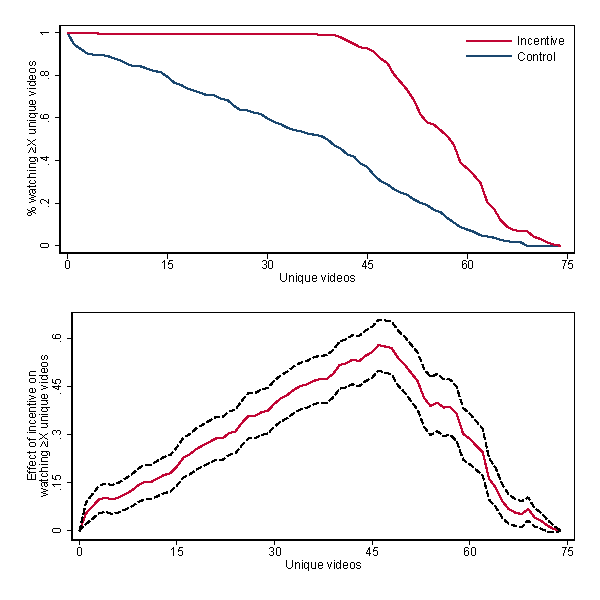
\includegraphics[width=1\textwidth, angle=0]{../plots/combo_cdf.pdf}
\footnotesize Top panels display the percent students in the \textit{Control}
 and \textit{Incentive} arms that watched at least $X$ unique videos (left) or hours of unique videos (right). Bottom panels display the differences between the two arms in the top panels with 95\% confidence intervals estimated by regressing an indicator for whether on the student watched at least $X\in\{0,...,X_{max}\}$ unique videos (or hours of unique videos) on the student's treatment status.
\end{center}
\end{figure}

% Time series: videos over time
\clearpage
\begin{figure}[t]
\begin{center}
\caption{Weekly video watching by treatment arm}
\label{timeseries}
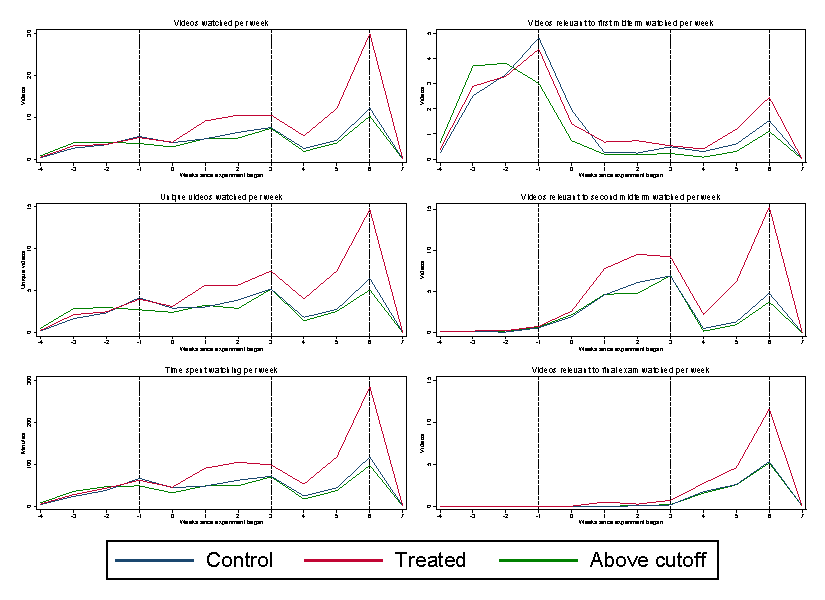
\includegraphics[width=1\textwidth, angle=0]{../plots/tscombo.pdf}
\footnotesize Dashed lines represent Midterm 1, Midterm 2, and Final exams
\end{center}
\end{figure}

% Regression discontinuity: midterm 2 exam scores
\clearpage
\begin{figure}[t]
\begin{center}
\caption{Regression Discontinuity: effect of treatment on videos watched and second midterm exam scores}
\label{rdmid2}
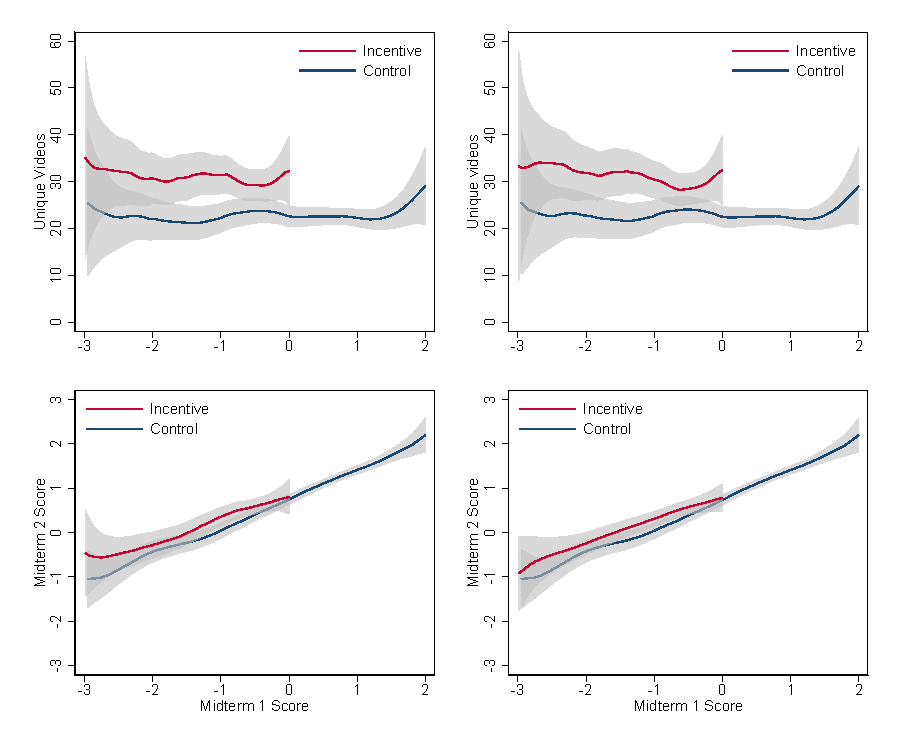
\includegraphics[width=1\textwidth, angle=0]{../plots/lpolymid2.pdf}
\footnotesize Videos (top) includes unique videos watched before the second midterm exam. Exam scores (bottom) are measured in control standard deviations. Confidence bands represent 95\% confidence intervals of the conditional mean outcome. The left plots includes all students who took the second midterm while the right plots exclude any students whose matched pair attrited.
\end{center}
\end{figure}

% Regression discontinuity: final exam scores
\clearpage
\begin{figure}[t]
\begin{center}
\caption{Regression Discontinuity: effect of treatment on videos watched and final exam scores}
\label{rdfinal}
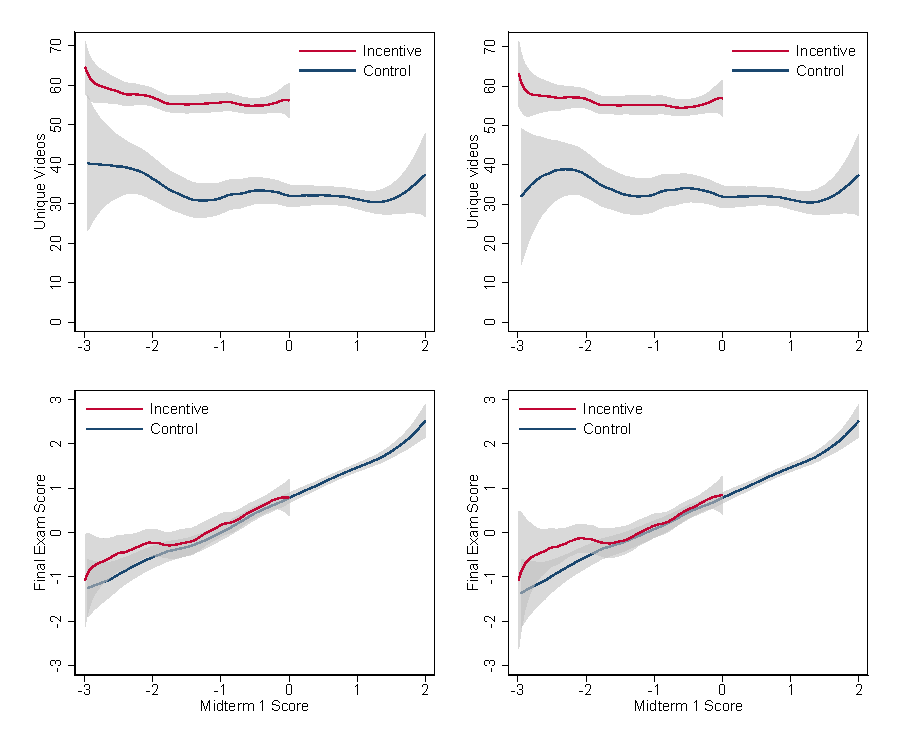
\includegraphics[width=1\textwidth, angle=0]{../plots/lpolyfinal.pdf}
\footnotesize Videos (top) includes unique videos watched before the final exam. Exam scores (bottom) are measured in control standard deviations. Confidence bands represent 95\% confidence intervals of the conditional mean outcome. The left plots includes all students who took the final exam while the right plots exclude any students whose matched pair attrited.
\end{center}
\end{figure}

% video CDF
\clearpage
\begin{figure}[t]
\begin{center}
\caption{Video watch rates by video and treatment arm, grouped by incentive}
\label{video_cdf}
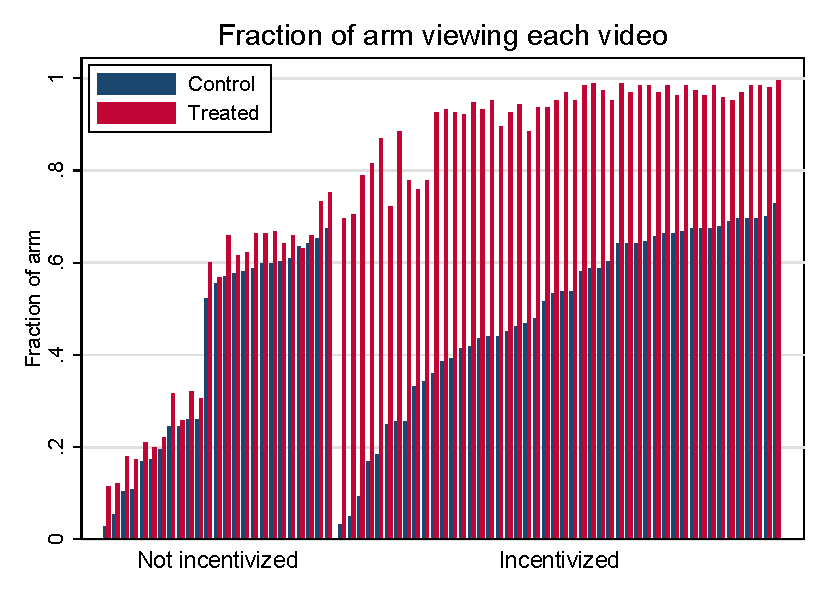
\includegraphics[width=1\textwidth, angle=0]{../plots/bar_uviews.pdf}
\footnotesize Each bar represents the fraction of the treatment arm that watched a particular video. Bars are in order of control group watch rates separately for incentivized and non-incentivized videos.
\end{center}
\end{figure}

\clearpage
\begin{figure}[t]
\begin{center}
\caption{Video watch rates by video and treatment arm, grouped by week}
\label{video_cdf_week}
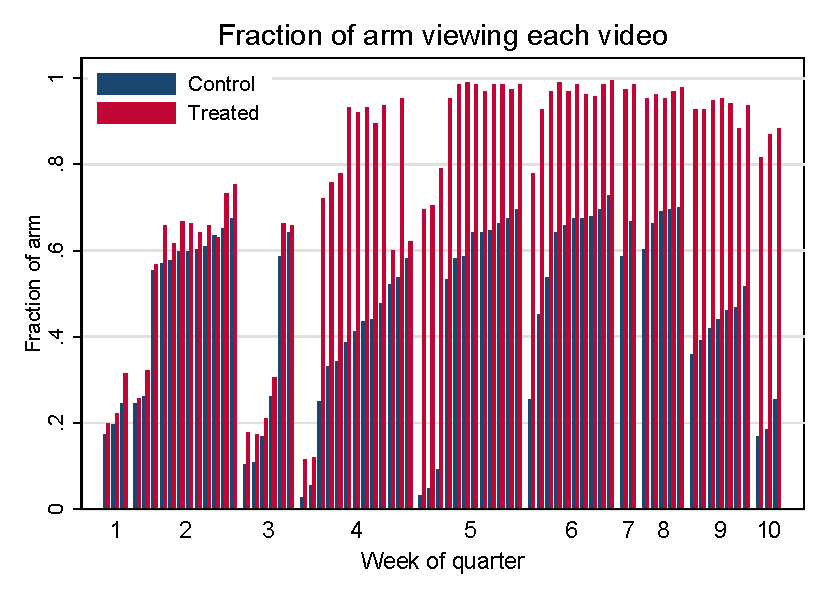
\includegraphics[width=1\textwidth, angle=0]{../plots/bar_uviews_week.pdf}
\footnotesize Each bar represents the fraction of the treatment arm that watched a particular video. Bars are in order of control group watch rates separately for each week the corresponding content was covered in lecture, as listed in the syllabus.
\end{center}
\end{figure}


% *****************************************************************
% Appendix
% *****************************************************************

\clearpage

\section*{Appendix}

\renewcommand{\thesubsection}{\Alph{subsection}}

\setcounter{table}{0}
\renewcommand{\thetable}{A\arabic{table}}
\setcounter{figure}{0}
\renewcommand{\thefigure}{A\arabic{figure}}

\subsection{Additional experiment details}

In this section we outline additional experiment details that could prove useful for replication or understanding our analysis choices.

\subsubsection{Randomization} \label{a_randomization}
Students were assigned to treatment arms using a matched pairs design, a special case of blocked randomization in which each block contains exactly two units, one treated and one control. Several authors detail how matched pair designs can improve the \textit{ex ante} precision of treatment effect estimates (versus complete randomization) by matching treatment units whose potential outcomes are similar (e.g. \cite{ir2015}, \cite{ai2017}).

Additionally, we were unable to observe most pretreatment covariates until after the experiment had concluded because of student privacy considerations, thereby making it impossible to block on these variables. We learned from the previous cohorts' data that between the first midterm score and math quiz score, both observable at the time of randomization, the midterm score predicted significantly more variation in the final exam score. Hence, we stratified on midterm score when assigning treatment. While we could have used an alternative method (e.g. matching methods) that take into consideration multiple covariates when assigning treatment, we opted for a simpler design given the high correlation between midterm and math quiz score and the comparatively high number of missing observations for the latter assessment (the math quiz was given on the second class day and so before some students enrolled in the class).

We assigned treatment shortly after issuing the first midterm exam grades, which occurred during the fourth week of the quarter. To assign treatment, we ordered the students by exam score, then paired students along this ordering for students below the median. Within pairs, we randomly assigned one student to \textit{Incentive}, the other to \textit{Control}. By construction, these two arms were \textit{ex ante} balanced on midterm exam score, and we verified at time of treatment that the arms were also balanced on math quiz score. Since this randomization was performed independently across year cohorts, by construction, the samples were also balanced on year.

Although our treatment assignment method provides a better chance of balance than does simple random sampling, by random chance and through non-random attrition, it is possible that the two treatment arms vary on \textit{ex post} observable and unobservable covariates that are correlated with the outcomes of interest, thereby confounding our treatment effect estimates. The primary cause of attrition was withdrawing from the course, which reduced our experiment sample by 35 students before the second midterm and an additional 21 students before the final exam. A 13\% withdraw rate is in line with the withdraw rates observed in previous quarters. Another cause of attrition, albeit not from the course, is age: four students under the age of 18 during the experiment were removed from the analysis dataset. Additionally, seven students opted out of having their data included in the experiment analysis.

Since neither the students' intent to withdraw, age, nor opt-out preferences were observable at the time of treatment assignment, we could not \textit{ex ante} balance this attrition across treatment arms. If students attrited non-randomly, that is, decided to attrite depending on their treatment status, then our treatment effect estimates would be biased. Fortunately, despite 8\% attrition before the second midterm and 13\% before the final exam, the two treatment arms below the median are balanced on nearly all observable pretreatment covariates, as shown in Tables \ref{balance_table_final} and \ref{balance_table_mid2}, which gives us confidence that the \textit{Control} arm is a good counterfactual for the \textit{Incentive} arm.

\subsubsection{Selection of control variables} \label{a_selection}

In this section we discuss how we select control variables included in our linear models.
% In our nonparametric estimation strategies that use generalized random forests, the algorithms implicitly select control variables that matter most for treatment heterogeneity and explaining variance in the outcome variables of interest (see Appendix \ref{a_grf}).

Equation \ref{itt_spec} includes a vector of control variables related linearly to the outcomes of interest. Although $d_i$, the treatment indicator is randomly assigned and in expectation $d_i$ is orthogonal to all observed and unobserved pretreatment covariates, in small samples stochastic imbalances can occur, which if controlled for can reduce bias of the treatment effect estimator \parencite{ai2017}. Even if perfect balance is achieved, controlling for orthogonal covariates can improve precision of the treatment effect estimator if the covariates can predict unexplained variance in the outcome.

By definition it is not possible to guarantee balance on unobserved covariates. As discussed in Appendix \ref{a_randomization}, we mechanically balanced the treatment arms on first midterm score, one of the few observables at the time of treatment assignment, with our knowledge from previous cohorts' data that the first midterm score explains a significant amount of variance in final exam score. Hence, in our estimation strategies including controls, we always include the first midterm score and year, following the recommendations of \textcite{bm2009} to control for all covariates used to seek balance when assigning treatment.

For variables unobservable at time of randomization but observable at time of analysis, we lack the luxury of guaranteed balance by construction, nor is it clear \textit{ex ante}, beyond our intuition, which will predict variation in the outcome variables of interest. On one hand, failing to control for valid predictors reduces statistical power. On the other hand, hand-picking control variables increases researcher degrees of freedom, risking increasing the prevalence of Type I errors \parencite{sns2011}. As such, in addition to a model without controls beyond the ones used for treatment assignment (year and midterm score), we fit a second model that includes a vector of linear controls chosen using the post-double-selection (PDS) procedure introduced by \textcite{bch2014a}.

PDS is a two step process in which first, model covariates are selected in an automated, principled fashion, and second, the model coefficients of interest are estimated while controlling for those selected covariates. The first step involves predicting, separately, both the outcome of interest (e.g., videos watched) and treatment status using lasso regression, which shrinks coefficient estimates towards zero. Note that since treatment is randomly assigned, the lasso should shrink most, if not all, of the coefficients towards zero when predicting treatment status. Next, the researcher takes the union of all covariates with non-zero coefficients and includes these covariates as controls in her model. With her control variables selected, she can now estimate treatment effects with reduced bias relative to including controls with less empirical rationale.

In Table \ref{controlvars_desc}, we describe all covariates observable in our study. In Table \ref{controlvars_selected_itt}, we describe the covariates selected as controls for estimating the effect of treatment on each outcome variable of interest. All models include either pair fixed effects or year and midterm score as controls. To ensure these controls are ``selected" by the PDS procedure, we partialed out these controls from the first step prediction models by residualizing both sides of the equation as described in \textcite{bch2014b}.

\subsection{LATE estimators using Neyman's repeated sampling approach} \label{a_neyman_late}

In this section we derive LATE estimators using the repeated sampling approach of \textcite{neyman1923}, which considers each pair as an independent, completely randomized experiment.

Similar to a Wald estimator, the point estimate of the LATE is the mean within-pair difference in outcome divided by the mean within-pair difference in videos:

\begin{equation} \label{neyman_late_spec}
	\wh{\gamma} = \frac{\wb{\Delta y}}{\wb{\Delta v}} = \frac{\frac{1}{J}\sum_{j=1}^{J} \Delta y_j }{\frac{1}{J}\sum_{j=1}^{J} \Delta v_j} = \frac{\wb{y_I} - \wb{y_C}}{\wb{v_I} - \wb{v_C}}
\end{equation}

where $y$ is the outcome of interest (grades) and $v$ is the number of videos, both indexed by pair $j\in J$ and treatment status $C$ or $I$ for \textit{Control} or \textit{Incentive}, respectively.

We use the delta method to calculate the approximate standard error of $\wh{\gamma}$. First, we define the following normally-distributed random variables:
\begin{equation}
\begin{split}
Y = \wb{y_I} - \wb{y_C} \sim \mathcal{N}(\mu_Y, \sigma^2_Y) \\
V = \wb{v_I} - \wb{v_C} \sim \mathcal{N}(\mu_V, \sigma^2_V)
\end{split}
\end{equation}

Using a first-order Taylor expansion and letting $g() = \frac{Y}{V}$, we have:
\begin{equation}
\begin{split}
	\text{Var}(g) & = \operatorname{E}[(g - \operatorname{E}(g))^2] \\
	& \approx \operatorname{E}[(g(\theta) + (Y-\theta_Y)g'_Y(\theta) + (V-\theta_V)g'_V(\theta) - g(\theta))^2] \\
	& = \operatorname{E}[(Y-\theta_Y)^2 (g'_Y(\theta))^2 + (V-\theta_V)^2 (g'_V(\theta))^2 + 2(Y-\theta_Y)(V-\theta_V)g'_Y(\theta)g'_V(\theta)] \\
	& = \text{Var}(Y)(g'_Y(\theta))^2 + \text{Var}(V)(g'_V(\theta))^2 + 2\text{Cov}(Y,V)g'_Y(\theta)g'_V(\theta)
\end{split}
\end{equation}

Expanding about $\theta=(\theta_Y,\theta_V)=(\mu_Y,\mu_V)$ and letting $g'_Y(\theta) = \mu_V^{-1}$ and $g'_V(\theta) = \frac{-\mu_Y}{\mu_V^{-2}}$:
\begin{equation} \label{var_expanded}
\begin{split}
	\text{Var}(g) & \approx \frac{1}{\mu_V^2}\text{Var}(Y) + \frac{\mu_Y^2}{\mu_V^4}\text{Var}(V) + 2\frac{-\mu_Y}{\mu_V^{-2}}\text{Cov}(Y,V) \\
	& = \frac{\mu_Y^2}{\mu_V^2}(\frac{\sigma_Y^2}{\mu_Y^2} + \frac{\sigma_V^2}{\mu_V^2} - 2\frac{\text{Cov}(Y,V)}{\mu_Y \mu_V})
\end{split}
\end{equation}

We use the following variance estimators of $Y$ and $V$ from Equation \ref{se_imai}:
\begin{equation}
\begin{split}
\wh{\text{Var}(Y)} & = \wh{\sigma_Y^2} = \frac{1}{J(J-1)}\sum_{j=1}^{J} (\Delta y_j - \wb{\Delta y})^2 \\
\wh{\text{Var}(V)} & = \wh{\sigma_V^2} = \frac{1}{J(J-1)}\sum_{j=1}^{J} (\Delta v_j - \wb{\Delta v})^2 \\
\wh{\text{Cov}(Y,V)} & = \wh{\sigma_{YV}} = \frac{1}{J(J-1)}\sum_{j=1}^{J} (\Delta y_j - \wb{\Delta y})(\Delta v_j - \wb{\Delta v})
\end{split}
\end{equation}

and the following estimators for the population means of $Y$ and $V$:
\begin{equation}
\begin{split}
\wh{\mu_Y} & = \operatorname{E}(\mu_Y) = \wb{\Delta y} \\
\wh{\mu_V} & = \operatorname{E}(\mu_V) = \wb{\Delta v}
\end{split}
\end{equation}

Substituting these variance and means estimators into the final step of \ref{var_expanded}, we arrive at the standard error estimator for $\wh{\gamma}$:

\begin{equation}
	\wh{\sigma_{\gamma}} = \frac{\wb{\Delta y}}{\wb{\Delta v}} \sqrt{ \frac{\wh{\sigma_Y^2}}{\wb{\Delta y}^2} + \frac{\wh{\sigma_V^2}}{\wb{\Delta v}^2} - 2 \frac{\wh{\sigma_{YV}}}{\wb{\Delta y} \wb{\Delta v}} }
\end{equation}

\clearpage
\begin{spacing}{1.0} 
\begin{table} \centering \caption{Baseline balance test, Midterm 2 sample} 
\label{balance_table_mid2} 
\resizebox{\linewidth}{!}{% 
\begin{threeparttable} 
\begin{tabular}{m{0.25\linewidth} *{7}{>{\centering\arraybackslash}m{0.095\linewidth}}}
\toprule 
 & \multicolumn{3}{c}{All students} & P-values & \multicolumn{2}{c}{Matched pairs}  & P-values  \\ 
 \cmidrule(lr){2-4}\cmidrule(lr){6-7} 

             Variable & Above Median &  Control & Incentive & (3) - (2) &  Control & Incentive & (5) - (4) \\
\midrule
      \customlinespace Midterm 1 score &        2.048 &    0.116 &     0.037 &     0.398 &    0.139 &     0.131 &     0.933 \\
                      &      (0.025) &  (0.063) &   (0.068) &           &  (0.065) &   (0.066) &           \\
          \customlinespace Year = 2019 &        0.492 &    0.513 &     0.500 &     0.797 &    0.514 &     0.514 &     1.000 \\
                      &      (0.025) &  (0.036) &   (0.035) &           &  (0.037) &   (0.037) &           \\
       \customlinespace Cumulative GPA &        3.445 &    2.944 &     2.948 &     0.965 &    2.942 &     2.992 &     0.487 \\
                      &      (0.029) &  (0.043) &   (0.058) &           &  (0.045) &   (0.056) &           \\
          \customlinespace No cum. GPA &        0.230 &    0.368 &     0.332 &     0.452 &    0.365 &     0.320 &     0.377 \\
                      &      (0.021) &  (0.035) &   (0.033) &           &  (0.036) &   (0.035) &           \\
      \customlinespace Math quiz score &        0.592 &    0.037 &     0.106 &     0.471 &    0.054 &     0.137 &     0.396 \\
                      &      (0.044) &  (0.070) &   (0.065) &           &  (0.071) &   (0.068) &           \\
          \customlinespace PSET visits &        0.269 &    0.259 &     0.223 &     0.655 &    0.276 &     0.232 &     0.612 \\
                      &      (0.042) &  (0.059) &   (0.056) &           &  (0.062) &   (0.061) &           \\
       \customlinespace Videos watched &       13.228 &   13.368 &    13.777 &     0.750 &   13.663 &    13.729 &     0.961 \\
                      &      (0.681) &  (0.886) &   (0.931) &           &  (0.929) &   (0.986) &           \\
       \customlinespace Videos, unique &        9.746 &    9.689 &    10.188 &     0.554 &    9.845 &    10.116 &     0.760 \\
                      &      (0.431) &  (0.580) &   (0.611) &           &  (0.606) &   (0.644) &           \\
         \customlinespace Hours videos &        1.690 &    1.782 &     1.825 &     0.818 &    1.827 &     1.804 &     0.906 \\
                      &      (0.093) &  (0.127) &   (0.135) &           &  (0.133) &   (0.142) &           \\
 \customlinespace Hours videos, unique &        1.291 &    1.355 &     1.387 &     0.802 &    1.382 &     1.364 &     0.897 \\
                      &      (0.062) &  (0.090) &   (0.092) &           &  (0.095) &   (0.096) &           \\
                \customlinespace Asian &        0.700 &    0.694 &     0.668 &     0.581 &    0.713 &     0.652 &     0.215 \\
                      &      (0.022) &  (0.033) &   (0.033) &           &  (0.034) &   (0.036) &           \\
               \customlinespace Latinx &        0.060 &    0.135 &     0.158 &     0.506 &    0.133 &     0.166 &     0.377 \\
                      &      (0.012) &  (0.025) &   (0.026) &           &  (0.025) &   (0.028) &           \\
                \customlinespace White &        0.151 &    0.114 &     0.124 &     0.765 &    0.105 &     0.138 &     0.336 \\
                      &      (0.018) &  (0.023) &   (0.023) &           &  (0.023) &   (0.026) &           \\
      \customlinespace Other ethnicity &        0.089 &    0.057 &     0.050 &     0.741 &    0.050 &     0.044 &     0.804 \\
                      &      (0.014) &  (0.017) &   (0.015) &           &  (0.016) &   (0.015) &           \\
               \customlinespace Female &        0.393 &    0.342 &     0.391 &     0.312 &    0.343 &     0.392 &     0.328 \\
                      &      (0.024) &  (0.034) &   (0.034) &           &  (0.035) &   (0.036) &           \\
                 \customlinespace Male &        0.592 &    0.653 &     0.604 &     0.316 &    0.652 &     0.602 &     0.329 \\
                      &      (0.024) &  (0.034) &   (0.034) &           &  (0.036) &   (0.036) &           \\
             \customlinespace Transfer &        0.271 &    0.477 &     0.455 &     0.673 &    0.470 &     0.436 &     0.528 \\
                      &      (0.022) &  (0.036) &   (0.035) &           &  (0.037) &   (0.037) &           \\
         \midrule 
 Observations &          417 &      193 &       202 &           &      181 &       181 &           \\
\bottomrule
\end{tabular}
\Fignote{This table includes all students who completed the second midterm. Descriptions of each variable can be found in Table \ref{controlvars_desc}. \textit{Male} and \textit{Female} do not include nine students who do not report a gender. \textit{P-values} are reported for the Welch's t-test of equal means between the \textit{Control} and \textit{Incentive} arms. \Regnote} 
\end{threeparttable}}
\end{table} 
\end{spacing}

\clearpage
\begin{spacing}{1.0} 
\begin{table} \centering \caption{Baseline balance test, Final Exam sample} 
\label{balance_table_final} 
\resizebox{\linewidth}{!}{% 
\begin{threeparttable} 
\begin{tabular}{m{0.25\linewidth} *{7}{>{\centering\arraybackslash}m{0.095\linewidth}}}
\toprule 
 & \multicolumn{3}{c}{All students} & P-values & \multicolumn{2}{c}{Matched pairs}  & P-values  \\ 
\cmidrule(lr){2-4}\cmidrule(lr){6-7} 

             Variable & Above Median &  Control & Incentive & (3) - (2) &  Control & Incentive & (5) - (4) \\
\midrule
      \customlinespace Midterm 1 score &        2.049 &    0.153 &     0.057 &     0.291 &    0.177 &     0.170 &     0.938 \\
                      &      (0.025) &  (0.061) &   (0.069) &           &  (0.064) &   (0.065) &           \\
          \customlinespace Year = 2019 &        0.489 &    0.516 &     0.500 &     0.753 &    0.518 &     0.518 &     1.000 \\
                      &      (0.025) &  (0.037) &   (0.036) &           &  (0.039) &   (0.039) &           \\
       \customlinespace Cumulative GPA &        3.445 &    2.946 &     2.959 &     0.864 &    2.929 &     3.001 &     0.346 \\
                      &      (0.029) &  (0.044) &   (0.060) &           &  (0.047) &   (0.059) &           \\
          \customlinespace No cum. GPA &        0.231 &    0.359 &     0.332 &     0.583 &    0.367 &     0.313 &     0.299 \\
                      &      (0.021) &  (0.035) &   (0.034) &           &  (0.038) &   (0.036) &           \\
      \customlinespace Math quiz score &        0.599 &    0.071 &     0.152 &     0.396 &    0.061 &     0.157 &     0.338 \\
                      &      (0.043) &  (0.068) &   (0.066) &           &  (0.071) &   (0.071) &           \\
      \customlinespace Tutoring visits &        0.270 &    0.272 &     0.237 &     0.684 &    0.283 &     0.253 &     0.746 \\
                      &      (0.043) &  (0.061) &   (0.060) &           &  (0.066) &   (0.066) &           \\
       \customlinespace Videos watched &       13.292 &   13.418 &    13.658 &     0.856 &   13.729 &    13.789 &     0.966 \\
                      &      (0.682) &  (0.909) &   (0.953) &           &  (0.978) &   (1.023) &           \\
       \customlinespace Videos, unique &        9.793 &    9.783 &    10.111 &     0.704 &    9.795 &    10.181 &     0.674 \\
                      &      (0.432) &  (0.598) &   (0.622) &           &  (0.630) &   (0.665) &           \\
         \customlinespace Hours videos &        1.698 &    1.788 &     1.805 &     0.929 &    1.812 &     1.803 &     0.967 \\
                      &      (0.094) &  (0.130) &   (0.138) &           &  (0.138) &   (0.148) &           \\
 \customlinespace Hours videos, unique &        1.297 &    1.369 &     1.372 &     0.985 &    1.363 &     1.366 &     0.985 \\
                      &      (0.062) &  (0.093) &   (0.094) &           &  (0.098) &   (0.100) &           \\
                \customlinespace Asian &        0.701 &    0.696 &     0.653 &     0.376 &    0.711 &     0.633 &     0.129 \\
                      &      (0.022) &  (0.034) &   (0.035) &           &  (0.035) &   (0.038) &           \\
               \customlinespace Latinx &        0.060 &    0.141 &     0.158 &     0.654 &    0.139 &     0.169 &     0.448 \\
                      &      (0.012) &  (0.026) &   (0.027) &           &  (0.027) &   (0.029) &           \\
                \customlinespace White &        0.149 &    0.109 &     0.132 &     0.497 &    0.102 &     0.145 &     0.244 \\
                      &      (0.018) &  (0.023) &   (0.025) &           &  (0.024) &   (0.027) &           \\
      \customlinespace Other ethnicity &        0.089 &    0.054 &     0.058 &     0.882 &    0.048 &     0.054 &     0.804 \\
                      &      (0.014) &  (0.017) &   (0.017) &           &  (0.017) &   (0.018) &           \\
               \customlinespace Female &        0.393 &    0.348 &     0.405 &     0.253 &    0.337 &     0.404 &     0.212 \\
                      &      (0.024) &  (0.035) &   (0.036) &           &  (0.037) &   (0.038) &           \\
                 \customlinespace Male &        0.593 &    0.647 &     0.584 &     0.215 &    0.657 &     0.584 &     0.176 \\
                      &      (0.024) &  (0.035) &   (0.036) &           &  (0.037) &   (0.038) &           \\
             \customlinespace Transfer &        0.272 &    0.462 &     0.447 &     0.778 &    0.470 &     0.416 &     0.321 \\
                      &      (0.022) &  (0.037) &   (0.036) &           &  (0.039) &   (0.038) &           \\
         
\midrule 
Observations &          415 &      184 &       190 &           &      166 &       166 &           \\
\bottomrule
\end{tabular}
\Fignote{This table includes all students who completed the final exam. Descriptions of each variable can be found in Table \ref{controlvars_desc}. \textit{Male} and \textit{Female} are coded zero for nine students who do not report a gender. \textit{P-values} are reported for the Welch's t-test of equal means between the \textit{Control} and \textit{Incentive} arms. \Regnote} 
\end{threeparttable}}
\end{table} 
\end{spacing}

\clearpage
\begin{spacing}{1.0}
\begin{table} \centering \caption{Anderson-Rubin confidence sets}
\label{arci_table}
\begin{threeparttable}
\begin{tabular}{ ccc }
\toprule
Outcome variable & Endogenous variable & Anderson-Rubin CI \\
\midrule
Midterm 2 score & 10 unique videos & [-0.001, 0.653] \\
Midterm 2 score & 1 hour videos & [-0.001, 0.392] \\
Final exam score & 10 unique videos & [0.000, 0.163] \\
Final exam score & 1 hour videos & [0.000, 0.102] \\
\bottomrule
\end{tabular}
\Fignote{This table displays Anderson-Rubin confidence sets at the 95\% confidence level for the 2SLS estimator $\hat{\gamma}$ from Equation \ref{secondstage_spec} including year dummies and first midterm score as controls. Outcomes are measured in standard deviations. Instrumented endogenous variables are measured in 10s of unique videos or hours of unique content.}
\end{threeparttable}
\end{table}
\end{spacing}

% Treatment effect heterogeneity
\clearpage
\begin{spacing}{1.0} 
\begin{table} \centering \caption{Heterogeneous Effects of Treatment} 
\label{het_table} 
\begin{threeparttable} 
\begin{tabular}{m{0.40\linewidth} *{2}{>{\centering\arraybackslash}m{0.12\linewidth}}}
\toprule
        Interaction Variable & Midterm 2 & Final Exam \\
\midrule
             \customlinespace Midterm 1 score &     0.009 &      0.002 \\
                             &   (0.086) &    (0.095) \\
                 \customlinespace Year = 2019 &     0.068 &      0.017 \\
                             &   (0.181) &    (0.179) \\
         \customlinespace Pretreatment videos &     0.011 &     -0.004 \\
                             &   (0.007) &    (0.007) \\
 \customlinespace Pretreatment videos, unique &    0.020\sym{*} &      0.001 \\
                             &   (0.011) &    (0.011) \\
                    \customlinespace Transfer &    -0.139 &      0.130 \\
                             &   (0.183) &    (0.178) \\
                      \customlinespace Female &    -0.208 &    -0.322\sym{*} \\
                             &   (0.185) &    (0.188) \\
                       \customlinespace Asian &  -0.402\sym{**} &     -0.215 \\
                             &   (0.189) &    (0.180) \\
                      \customlinespace Latinx &     0.237 &      0.022 \\
                             &   (0.254) &    (0.227) \\
                       \customlinespace White &   0.638\sym{**} &      0.271 \\
                             &   (0.260) &    (0.250) \\
             \customlinespace Other ethnicity &    -0.113 &      0.276 \\
                             &   (0.307) &    (0.347) \\
                
\midrule 
Observations &       395 &        374 \\
\bottomrule
\end{tabular}
\Fignote{This table reports estimates for $\beta_2$ from Equation \ref{eq:het_spec}. Test scores are measured in standard deviation units. \Regnote}
\end{threeparttable}
\end{table} 
\end{spacing}

\clearpage
\begin{spacing}{1.0}
\begin{table} \centering \caption{Regression Discontinuity estimates}
\label{rdtable}
\begin{threeparttable}
\begin{tabular}{m{0.35\linewidth} *{3}{>{\centering\arraybackslash}m{0.1\linewidth}}}
\toprule
 & Control Mean & (1) & (2) \\
\midrule
\multicolumn{4}{l}{\textbf{Panel A}: Midterm 2} \\
\customlinespace \indentrow{Unique videos} & 22.7 & 9.12\sym{***} & 9.34\sym{***} \\
& & (3.35) & (3.42) \\
\customlinespace \indentrow{Midterm 2 score} & 0.73 & 0.06 & 0.07 \\
& & (0.20) & (0.19) \\
\midrule
Observations & & 812 & 779 \\
\midrule
\multicolumn{4}{l}{\textbf{Panel B}: Final exam} \\
\customlinespace \indentrow{Unique videos} & 32.0 & 24.16\sym{***} & 24.95\sym{***} \\
& & (2.39) & (2.48) \\
\customlinespace \indentrow{Final exam score} & 0.78 & 0.11 & 0.14 \\
& & (0.18) & (0.19) \\
\midrule
Observations & & 789 & 747 \\
\bottomrule
\end{tabular}
\Fignote{This table reports coefficients on $\tau(c)$ from Equations \ref{rd_spec}. Panel A includes Midterm 2-takers while Panel B includes Final Exam-takers. Model (1) includes all students while (2) contains only students whose pair did not attrite. Standard errors are in parentheses. ***, **, and * indicate significance at the 1, 5, and 10 percent critical levels, respectively.}
\end{threeparttable}
\end{table}
\end{spacing}

\clearpage
\begin{spacing}{1.0}\centering 
\begin{longtable}{p{0.3\linewidth} p{0.6\linewidth}}
\caption{Description of control variables eligible for selection a la Belloni et al (2014).}\label{controlvars_desc}\\
\toprule
        Variable &                                              Description \\
\midrule
\endhead
\midrule
\multicolumn{2}{r}{{Continued on next page}} \\
\midrule
\endfoot

\bottomrule
\endlastfoot
 Midterm 1 score &                               Score on the first midterm \\
     Year = 2019 &                   1 if course taken in 2019, 0 otherwise \\
  Cumulative GPA &        Cumulative GPA from prior term, 0 if not observed \\
     No cum. GPA &              1 if Cumulative GPA unobserved, 0 otherwise \\
 Math quiz score &       Score on a quiz assessing prerequisite math skills \\
     PSET visits &            Number of PSET visits as of the first midterm \\
  Videos watched &  Number of unique videos watched as of the first midterm \\
    Hours videos &   Hours of unique videos watched as of the first midterm \\
           Asian &                     1 if ethnicity is Asian, 0 otherwise \\
          Latinx &                    1 if ethnicity is Latinx, 0 otherwise \\
           White &                     1 if ethnicity is White, 0 otherwise \\
          Female &                                 1 if female, 0 otherwise \\
        Transfer &                       1 if transfer student, 0 otherwise \\
\end{longtable}
\end{spacing}

\clearpage
\begin{spacing}{1.0} 
\begin{ThreePartTable} 
\begin{TableNotes} 
\item \textit{Note}: Controls chosen via the PDS procedure of \textcite{bch2014a}. In the \textit{All Observations} model, \textit{Midterm 1 score} and \textit{Year = 2019} are additionally included as controls. In the \textit{Fixed Effects} model, pair fixed effects and \textit{Midterm 1 score} are included. All control variables are measured before the start of the experiment, e.g. \textit{Hours videos} is the hours of videos watched as of the first midterm.
\end{TableNotes} 
\footnotesize 
 \begin{longtable}{p{0.07\linewidth} >{\hangindent=1em}p{0.38\linewidth} p{0.22\linewidth} p{0.22\linewidth}}
\caption{ITT model controls selected via post-double-selection}\label{controlvars_selected_itt}\\
\toprule
      Table &                          Dependent Variable &                  Controls,\newline All Observations &                                                         Controls,\newline Fixed Effects \\
\midrule
\endfirsthead 
\multicolumn{4}{r}{{Table \ref{controlvars_selected_itt} (continued)}} \\
\toprule 
 \endhead
\midrule
\multicolumn{4}{r}{{Continued on next page}} \\
\midrule
\endfoot

\bottomrule
\insertTableNotes 
\endlastfoot
    Table 1 &                Hours unique videos by Final &                         Hours videos\newline Videos &                                                             Hours videos\newline Videos \\
            &               Hours unique videos by Mid. 2 &                                        Hours videos &                                                             Hours videos\newline Videos \\
            &                       Hours videos by Final &                                        Hours videos &                                                                            Hours videos \\
            &                      Hours videos by Mid. 2 &                                        Hours videos &                                         Hours videos\newline PSET visits\newline Videos \\
            &             Num. unique videos before Final &                         Hours videos\newline Videos &                                                                                  Videos \\
            &            Num. unique videos before Mid. 2 &                         Hours videos\newline Videos &                                                                                  Videos \\
            &                    Num. videos before Final &                         Hours videos\newline Videos &                                                             Hours videos\newline Videos \\
            &                   Num. videos before Mid. 2 &                         Hours videos\newline Videos &                                         Hours videos\newline PSET visits\newline Videos \\
    \midrule 
Table 2 &                            Final exam score &                                                None &                                                        Math quiz score\newline Transfer \\
            &                             Midterm 2 score &                                                None &                                                                         Math quiz score \\
    \midrule 
Table 3 &                                 All classes &                                      Cumulative GPA &                                 Cumulative GPA\newline Math quiz score\newline Transfer \\
            &                    Econ classes ex. Micro A &                                                None &                                                         Cumulative GPA\newline Transfer \\
            &                           Excluding Micro A &                                      Cumulative GPA &                                                                                Transfer \\
            &                      Excluding econ classes &                                                None &                                                                                    None \\
            &                     Letter grade in Micro A &      Cumulative GPA\newline Latinx\newline Transfer &                                                                          Cumulative GPA \\
            &                     Num. classes not passed &                                                None &                                                                                    None \\
            &                         Num. classes passed &                     Cumulative GPA\newline Transfer &                                                         Cumulative GPA\newline Transfer \\
            &                     Num. classes taken P/NP &                                              Latinx &                                                                                  Latinx \\
            &               Num. classes taken for letter &                  Cumulative GPA\newline No cum. GPA &                                                                          Cumulative GPA \\
            &                      Num. classes withdrawn &                                                None &                                                                                    None \\
            &                       Num. units taken P/NP &                                              Latinx &                                                                                  Latinx \\
            &           Num. units taken for letter grade &                  Cumulative GPA\newline No cum. GPA &                                                                          Cumulative GPA \\
            &                        Num. units withdrawn &                                                None &                                                                                    None \\
            &                       \% classes taken P/NP &                                                None &                                                                                  Latinx \\
            &                 \% classes taken for letter &                                                None &                                                                                  Latinx \\
    \midrule 
Table 4 &                           Attendance checks &  Female\newline Math quiz score\newline PSET visits &                                                                             PSET visits \\
            &                         Num. Piazza answers &                                                None &                                                                                    None \\
            &                     Num. Piazza days online &                                                None &                                                                                    None \\
            &                 Num. Piazza questions asked &                                                None &                                                                                    None \\
            &                           Num. Piazza views &                                                None &                                                                                   Asian \\
            &                         Num. of PSET visits &                                         PSET visits &                                                                             PSET visits \\
    \midrule 
Table 5 &                             Hours of videos &                                        Hours videos &  Hours videos\newline Latinx\newline Math quiz score\newline PSET visits\newline Videos \\
            &                             Midterm 1 score &                                                None &                                           Latinx\newline Math quiz score\newline Videos \\
            &                             Midterm 2 score &                                                None &                             Asian\newline Latinx\newline Math quiz score\newline Videos \\
            &                     Num. classes not passed &                                                None &                                                                                    None \\
            &                         Num. classes passed &                                                None &                                                                                    None \\
            &                     Num. classes taken P/NP &                                                None &                                                                                Transfer \\
            &               Num. classes taken for letter &                                                None &                                                                             No cum. GPA \\
            &                      Num. classes withdrawn &                                                None &                                                                                    None \\
            &                              Num. of videos &                                        Hours videos &  Hours videos\newline Latinx\newline Math quiz score\newline PSET visits\newline Videos \\
            &                       Num. units taken P/NP &                                                None &                                                                                Transfer \\
            &           Num. units taken for letter grade &                                                None &                                                                                    None \\
            &                        Num. units withdrawn &                                                None &                                                                                    None \\
            &                                    Term GPA &                                      Cumulative GPA &                                                      Cumulative GPA\newline PSET visits \\
            &  Term GPA, econ courses ex. Micro B, winter &                                                None &                                                                         Math quiz score \\
            &                       Term GPA, ex. Micro B &                                      Cumulative GPA &                                                      Cumulative GPA\newline PSET visits \\
            &                  Term GPA, ex. econ courses &                                                None &                                                                             PSET visits \\
            &                                Took Micro B &                                                None &                                                                         Math quiz score \\
            &                       \% classes taken P/NP &                                                None &                                                            No cum. GPA\newline Transfer \\
            &                 \% classes taken for letter &                                                None &                                                            No cum. GPA\newline Transfer \\
 Table None &                            Final exam score &                                                None &                                           Latinx\newline Math quiz score\newline Videos \\
            &                         Hours unique videos &                                        Hours videos &  Hours videos\newline Latinx\newline Math quiz score\newline PSET visits\newline Videos \\
            &                          Num. unique videos &                                        Hours videos &  Hours videos\newline Latinx\newline Math quiz score\newline PSET visits\newline Videos \\
            &                                Pass Micro B &                                                None &                                           Latinx\newline Math quiz score\newline Videos \\
\end{longtable}

\end{ThreePartTable} 
\end{spacing}

\clearpage
\begin{spacing}{1.0} 
\begin{table} \centering \caption{LATE model controls selected via post-double-selection} 
\label{controlvars_selected_iv} 
\resizebox{\linewidth}{!}{% 
\begin{threeparttable} 
\begin{tabular}{p{.25\linewidth} p{0.3\linewidth} p{0.22\linewidth} p{0.22\linewidth}}
\toprule
Dependent Variable &          Instrumented &                                           Controls,\newline All Observations & Controls,\newline Fixed Effects \\
\midrule
  Final exam score &  Hours videos, unique &         Hours videos\newline Math quiz score\newline Transfer\newline Videos &     Hours videos\newline Videos \\
  Final exam score &        Videos, unique &                                                  Hours videos\newline Videos &     Hours videos\newline Videos \\
   Midterm 2 score &  Hours videos, unique &  Hours videos\newline Math quiz score\newline Tutoring visits\newline Videos &                    Hours videos \\
   Midterm 2 score &        Videos, unique &                                                  Hours videos\newline Videos &     Hours videos\newline Videos \\
\bottomrule
\end{tabular}
\Fignote{Controls chosen via the PDS procedure of \textcite{bch2014a}. In the \textit{All Observations} model, \textit{Midterm 1 score} and \textit{Year = 2019} are additionally included as controls. In the \textit{Fixed Effects} model, pair fixed effects and \textit{Midterm 1 score} are included. All control variables are measured before the start of the experiment, e.g. \textit{Hours videos} is the hours of videos watched as of the first midterm.} 
\end{threeparttable}}
\end{table} 
\end{spacing}

%%% PLOTS

% Histogram of videos eligible for incentive
\clearpage
\begin{figure}[t]
\begin{center}
\caption{Distribution of videos counted towards incentive}
\label{hist_incent} % TODO add reference in paper
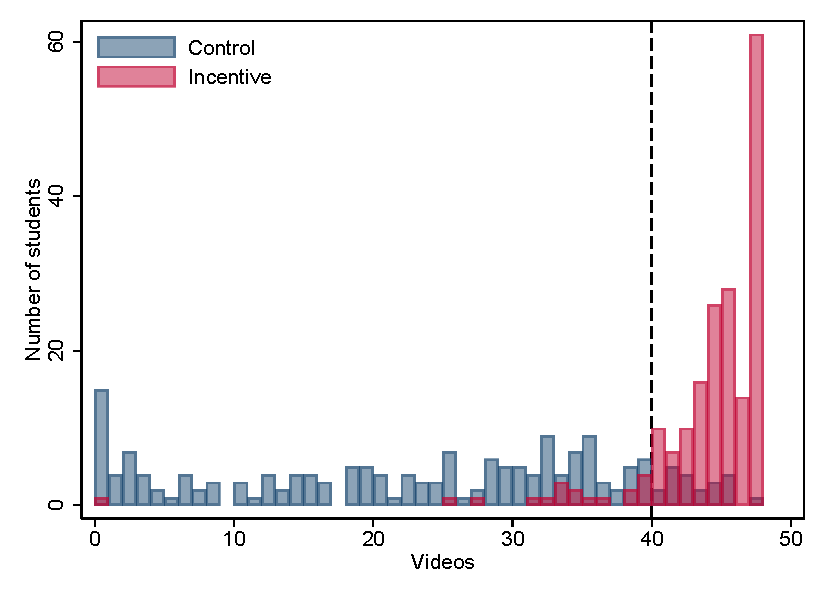
\includegraphics[width=1\textwidth, angle=0]{../plots/hist_v_incent.pdf}
\footnotesize This plot includes only videos that would have counted towards the earning the grade incentive. Students were required to watch 40 unique of 48 eligible videos between the first midterm and final exam to earn the grade incentive. 91\% of \textit{Incentive} students met the requirements for the grade incentive versus 11\% of \textit{Control} students.
\end{center}
\end{figure}

% Time series: videos over time by exam topic
% This shows that students watch videos when most useful
\clearpage
\begin{figure}[t]
\begin{center}
\caption{Weekly video watching by exam topic}
\label{timeseries_by_exam} % TODO add reference in paper
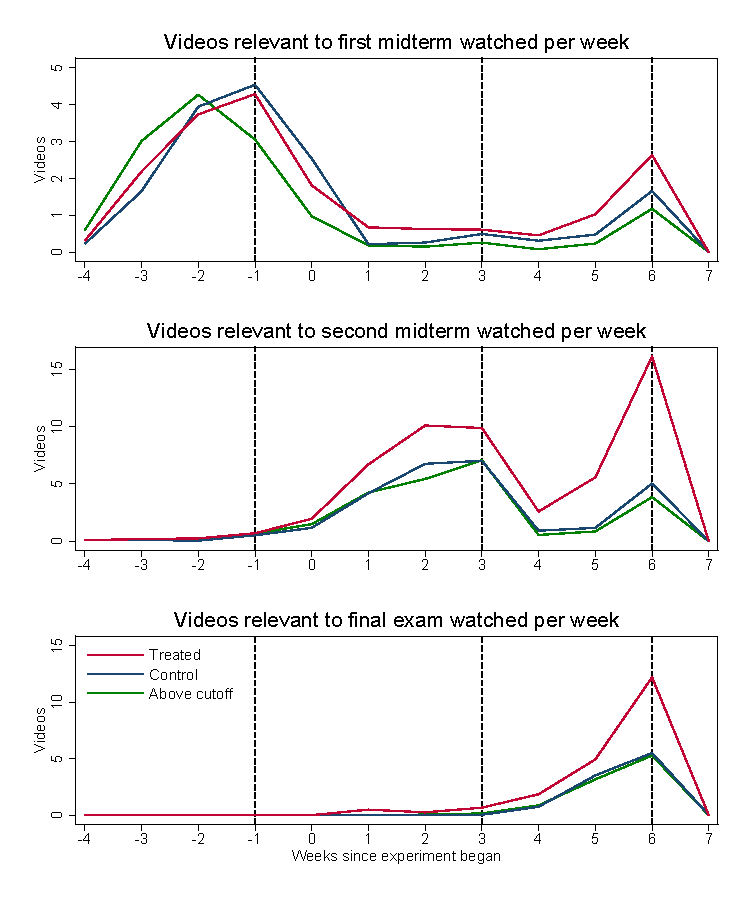
\includegraphics[width=1\textwidth, angle=0]{../plots/tscombo_exam.pdf}
\footnotesize Dashed lines represent Midterm 1, Midterm 2, and Final exams.
\end{center}
\end{figure}

% Treatment effects vs Midterm 1 score
% \clearpage
% \begin{figure}[t]
% \begin{center}
% \caption{Effect of treatment on videos watched and exam scores by Midterm 1 score}
% 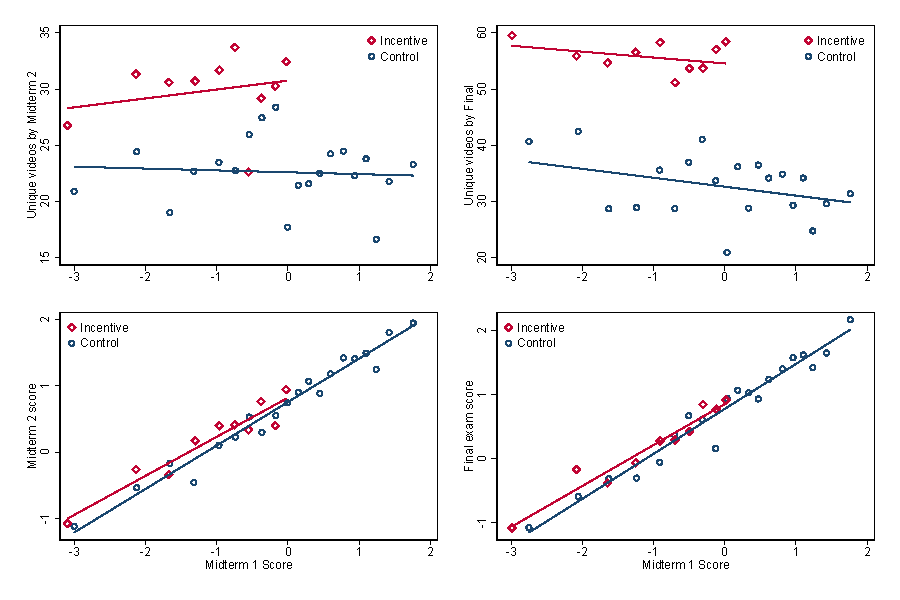
\includegraphics[width=1\textwidth, angle=0]{../plots/combo_binscatter.pdf}
% \footnotesize Test scores in standard deviation units. Each point comprises 5-percentile bins along the domain. The control points displayed include both \textit{Control} and \textit{Above median} arms.
% \end{center}
% \end{figure}

% Histogram of 'binge watching' - distribution of max(weekly videos watched)
\clearpage
\begin{figure}[t]
\begin{center}
\caption{Distribution of max videos watched in one week}
\label{hist_binge}
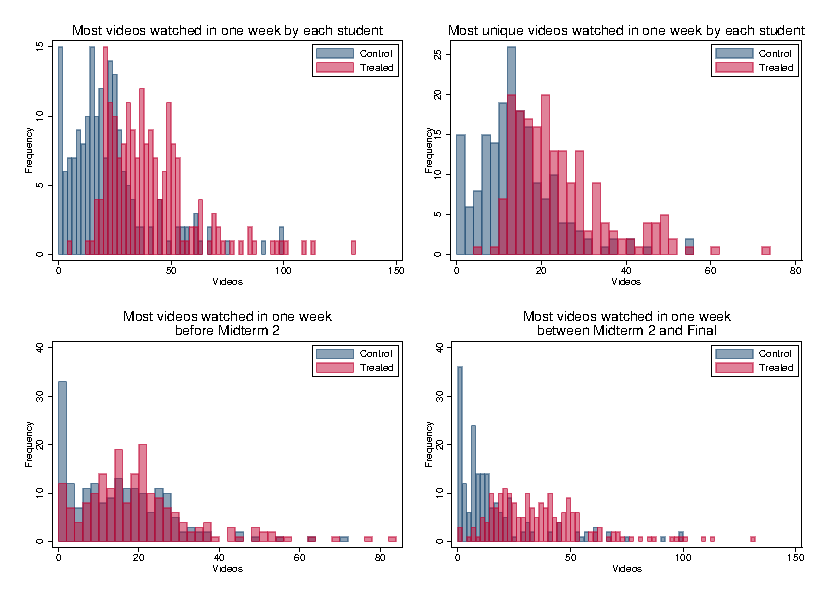
\includegraphics[width=1\textwidth, angle=0]{../plots/hist_maxweek.pdf}
\footnotesize These plots help illustrate potential ``binge watching" behavior. Compared to the \textit{Control} students, \textit{Incentive} students are more likely to watch 40 or more unique videos in a week, which occurs in the weeks preceding the final and not the second midterm.
\end{center}
\end{figure}

% Regression discontinuity: no manipulation
\clearpage
\begin{figure}[t]
\begin{center}
\caption{Distribution of Midterm 1 scores}
\label{mid1dist}
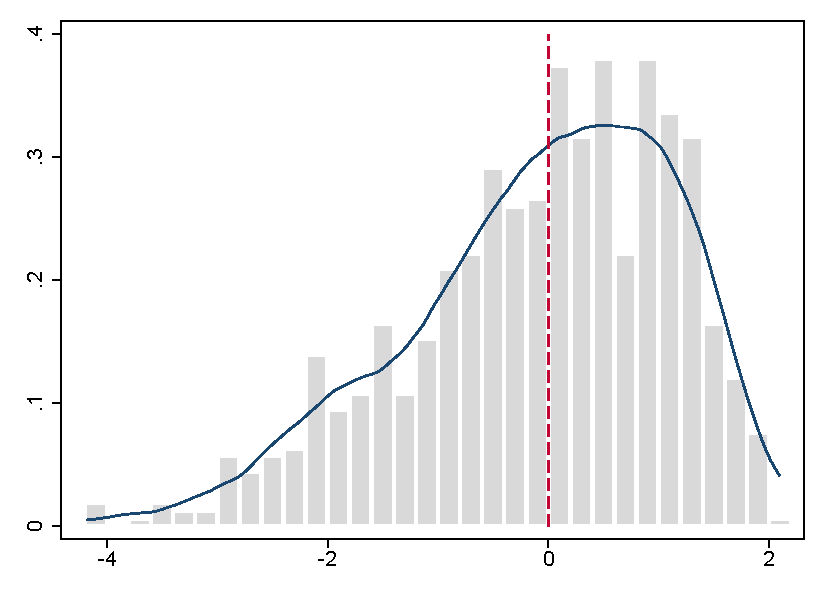
\includegraphics[width=1\textwidth, angle=0]{../plots/mid1dist.pdf}
\footnotesize Midterm scores are measured in control standard deviations. This histogram includes all students who took the final exam. As such, this plot would allow one to observe bunching if treatment caused differential attrition or manipulation of one's midterm score.
\end{center}
\end{figure}

% video CDF by duration
\clearpage
\begin{figure}[t]
\begin{center}
\caption{Video watch rates by video and treatment arm, grouped by incentive, ordered by video duration}
\label{video_cdf_duration}
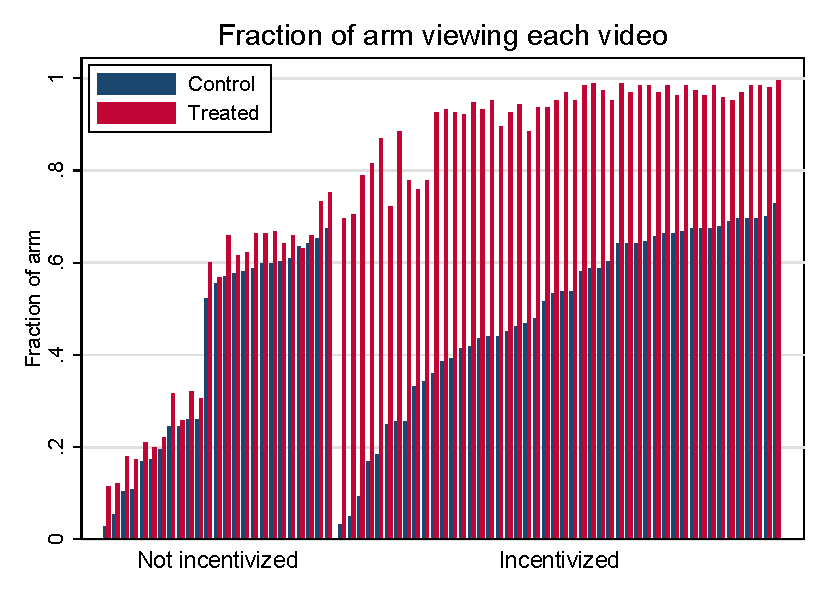
\includegraphics[width=1\textwidth, angle=0]{../plots/bar_uviews.pdf}
\footnotesize Each bar represents the fraction of the treatment arm that watched a particular video. Bars are in order of video duration separately for incentivized and non-incentivized videos.
\end{center}
\end{figure}


\end{document}

% \subsubsection{Generalized Random Forests} \label{a_grf}
%
% In this section we discuss our implementation of Generalized Random Forests proposed by \textcite{atw2019}
